\documentclass[
    reprint, 
    aps,
    preprintnumbers,
    twocolumn,
    prb,
    superscriptaddress
]{revtex4-2}


%=======================
% Packages:
%=======================

\usepackage[utf8]{inputenc}
\usepackage{booktabs}
\usepackage[multiple]{footmisc}
\usepackage{lipsum}
\usepackage{rotating}
\usepackage{perpage}
\usepackage{chronology}
\usepackage{lipsum}
\usepackage{amssymb}
\usepackage{amsbsy}
\usepackage{amsmath}
\usepackage{tikz}
\usepackage[T1]{fontenc}
\usepackage{etoolbox}
\usepackage{graphics}
\usepackage{abraces}
\makeatletter
\let\unit\relax % otherwise there are package conflicts with siunitx
\makeatother
\usepackage{siunitx}
\usepackage{hyperref}
%\usepackage{float}
\usepackage{multirow}
\usepackage{mathtools}
\usepackage{bm}
\usepackage{url}
\usepackage{physics}
\usepackage{hyperref}
\usepackage{bbm}
\usepackage{color}
\usepackage{placeins}
\usepackage[normalem]{ulem}
\usepackage{mhchem}

%=======================
% New Commands:
%=======================

\newcommand{\vk}{\vec{k}}
\newcommand{\vl}{\vec{l}}
\newcommand{\vQ}{\vec{Q}}
\newcommand{\up}{\uparrow}
\newcommand{\down}{\downarrow}
\newcommand{\kplusQ}{\vk+\vQ}
\newcommand{\kminusQ}{-\vk-\vQ}

\newcommand{\ddt}{\frac{\mathrm{d}}{\mathrm{d}t}}
\newcommand{\dgamma}{\mathrm{d}\gamma}

\newcommand{\mM}{\mathcal{M}}
\newcommand{\mN}{\mathcal{N}}

\newcommand{\greens}[1]{\mathcal{G}_\text{#1} (\omega)}
\newcommand{\spectral}[1]{\mathcal{A}_\text{#1}  (\omega)}

\begin{document} 

% Preliminary title
\title{Collective excitations in competing phases in two and three dimensions}

%=======================
% Authors:
%=======================

\author{Joshua Alth\"user}\email{joshua.althueser@tu-dortmund.de}
\affiliation{Condensed Matter Theory, TU Dortmund University,
Otto-Hahn Stra\ss{}e 4, 44221 Dortmund, Germany}

\author{G\"otz S.~Uhrig}
\email{goetz.uhrig@tu-dortmund.de}
\affiliation{Condensed Matter Theory, TU Dortmund University,
Otto-Hahn Stra\ss{}e 4, 44221 Dortmund, Germany}

\date{\today}

%%%%%%%%%%%%%%%%%%%%%%%%%%%%%%%%%%%%%%%%%%%%%%%%%%%%%%%%%%%%%%%%%%%%%%%%%%%%%%%%%%%%%%%%%%%%%%%%%%%%%%%%%%%%%%%%%%%%%
%%%%%%%%%%%%%%%%%%%%%%%%%%%%%%%%%%%%%%%%%%%%%%%%%%%%%%%%%%%%%%%%%%%%%%%%%%%%%%%%%%%%%%%%%%%%%%%%%%%%%%%%%%%%%%%%%%%%%
%%%%%                                                  Abstract                                                 %%%%%
%%%%%%%%%%%%%%%%%%%%%%%%%%%%%%%%%%%%%%%%%%%%%%%%%%%%%%%%%%%%%%%%%%%%%%%%%%%%%%%%%%%%%%%%%%%%%%%%%%%%%%%%%%%%%%%%%%%%%
%%%%%%%%%%%%%%%%%%%%%%%%%%%%%%%%%%%%%%%%%%%%%%%%%%%%%%%%%%%%%%%%%%%%%%%%%%%%%%%%%%%%%%%%%%%%%%%%%%%%%%%%%%%%%%%%%%%%%
\begin{abstract}
    We investigate the superconducting (SC), charge-density wave (CDW), and antiferromagnetic (AFM) phases 
    in the extended Hubbard model at zero temperature and half-filling.
    We employ the iterated equations of motion approach \cite{Kalthoff17,bleicker18} to compute the two-particle Green's functions and by extension, the corresponding spectral densities.
    This renders comprehensive analysis of the behavior of collective excitations possible as the model's parameters are changed across phase transitions.
    We identify the well-known amplitude (Higgs) and phase (Anderson-Bogoliubov) modes within the superconducting phase and observe a similar excitation in the CDW phase which shifts towards zero energy as the system approaches the phase transition to the SC phase.
    In the CDW phase, close to the phase transition to the AFM phase, we find a collective mode that does not change significantly and another mode that becomes soft as the phase boundary is approached.
\end{abstract}

\maketitle

%%%%%%%%%%%%%%%%%%%%%%%%%%%%%%%%%%%%%%%%%%%%%%%%%%%%%%%%%%%%%%%%%%%%%%%%%%%%%%%%%%%%%%%%%%%%%%%%%%%%%%%%%%%%%%%%%%%%%
%%%%%%%%%%%%%%%%%%%%%%%%%%%%%%%%%%%%%%%%%%%%%%%%%%%%%%%%%%%%%%%%%%%%%%%%%%%%%%%%%%%%%%%%%%%%%%%%%%%%%%%%%%%%%%%%%%%%%
%%%%%                                                Introduction                                               %%%%%
%%%%%%%%%%%%%%%%%%%%%%%%%%%%%%%%%%%%%%%%%%%%%%%%%%%%%%%%%%%%%%%%%%%%%%%%%%%%%%%%%%%%%%%%%%%%%%%%%%%%%%%%%%%%%%%%%%%%%
%%%%%%%%%%%%%%%%%%%%%%%%%%%%%%%%%%%%%%%%%%%%%%%%%%%%%%%%%%%%%%%%%%%%%%%%%%%%%%%%%%%%%%%%%%%%%%%%%%%%%%%%%%%%%%%%%%%%%

\section{Introduction}\label{sec:introduction}


The study of collective excitations is of great scientific interest as it sheds light on the intricate dynamics of correlated electron systems, providing crucial insights into emergent material properties.
On the theoretical side, the Hubbard model has been employed in a plethora of previous studies. 
Early studies proved the existence of eigenstates to the Hubbard Hamiltonian that exhibit off-diagonal long-range order,
encouraging the model's usage for the description of high-temperature superconductivity \cite{yang89}.
Shortly afterward, an exact SO(4) symmetry was discovered, which allows a degeneracy of superconductivity (SC) and a charge-density wave (CDW) governed by an attractive on-site interaction \cite{yang90}.
This coexistence can be argued by the existence of a particle-hole transformation on bipartite lattices, 
that maps the attractive Hubbard model exactly onto the repulsive one, exhibiting antiferromagnetism (AFM) \cite{Hirsch85}.
The previously mentioned SC and CDW phases map to different spin operators \cite{zitko15,lieb89}.

Numerous studies have investigated the phases and various quantities of the Hubbard model in equilibrium systems, including various additional interactions with and without doping.
\cite{Micnas88,Micnas88b,Micnas89,Dzierzawa92,Kostyrko92,Eriksson95,Staudt00,Onari04,Toschi05,Brackett16,Paki19,romer20,Sushchyev22}.
For a long time, research on the dynamics of the superconducting gap parameter focused on its behavior after an instantaneous quench, 
yielding damped or persistent oscillations depending on the magnitude of the quench \cite{Volkov73,Yuzbashyan05,Yuzbashyan06,Barankov06,Cui19}.
More recent experimental and theoretical studies examined the driven systems in the hope of inducing superconductivity \cite{Nicoletti14,Krull14,Moor14,Casandruc15,patel16,sentef17,Buenemann17}.

In this paper, we will restrict ourselves to the half-filled Hubbard model, including an additional intersite interaction, on a square and a simple cubic lattice.
The 2D case already exhibits a wide range of possible phases, including CDW, AFM, $s$- and $d_{x^2 - y^2}$-wave superconductivity, and phase-separated states \cite{Micnas88b,Tsuchiura95,Su01,Su04,ha11,Huang13,Jiang22,Linner23}.
We expand these well-known phase diagrams to the simple cubic lattice where we find a similar structure for CDW, AFM, and $s$-wave SC.

To study this system, we will first employ a mean-field approximation to the interaction terms 
and then use the methodology from the so-called iterated equations of motion approach (iEoM),
which has already seen success in the handling of interaction quenches \cite{uhrig09,hamerla13,hamerla14,bleicker18}.
Here, one commutes operators from a suitable operator basis with the Hamiltonian and adds the newly occurring terms to it.
Naturally, a truncation is necessary for most practical applications, however, the approximation becomes better the more terms are included within the basis.
The functionality of this method has been compared to the density matrix formalism and has proved to be considerably more accurate \cite{Kalthoff17}.

Moreover, we demonstrate an explicit way to obtain various Green's functions from the aforementioned methodology.
By extension, we also obtain the spectral functions of the investigated systems and discuss the excitations found therein.
The prominent examples in the SC phase are the well-known phase (Anderson-Bogoliubov) and amplitude (Higgs) modes \cite{Kulik1981,Varma02,Cea14,Measson14,Tsuji15,Krull16,Schwarz20,Fan22}.
The former is located at zero energy as our model describes neutral superfluids.
The latter is found at the lower edge of the two-particle continuum.

The remainder of this paper is organized as follows:
In \autoref{sec:model} we will introduce the model and its Hamiltonian as well as our mean-field theory for the ground state.
We give a brief overview of the iterated equations of motion approach and derive a rigorous link to Green's functions in \autoref{sec:ieom}.
Next, we show our results in \autoref{sec:results}.
Lastly, in \autoref{sec:conclusion}, we will discuss our results.

\section{Model and mean-field theory}\label{sec:model}

\subsection{Model}

In our study, we employ the extended Hubbard model as it encompasses assorted phases and thereby provides direct access to the rich excitation spectra therein.
Its Hamiltonian is given by
\begin{equation}
    \label{eqn:full_hamiltonian}
    \begin{aligned}
        H = &-t \sum_{\langle i, j \rangle, \sigma} \left( c_{i\sigma}^\dagger c_{j\sigma} + \text{h.c.} \right) 
        + \mu \sum_{i,\sigma} n_{i\sigma} \\
        &+ U \sum_{i} n_{i\uparrow} n_{i\downarrow} 
        + \frac{V}{2} \sum_{\langle i, j\rangle, \sigma} n_{i\sigma} n_{j\sigma}\,,
    \end{aligned}
\end{equation}
where $c_{i\sigma}^{(\dagger)}$ annihilates (creates) an electron with spin $\sigma$ on lattice site $i$ 
and $\langle i, j\rangle$ denotes the summation over the next neighbors.
The parameters are the hopping amplitude $t$, the onsite interaction $U$, the intersite interaction $V$, and the chemical potential $\mu$.
Applying a Fourier transform into $k$ space yields the single-particle dispersion 
\begin{equation}
    \epsilon_0 (\vk) = -2t \sum_{\alpha=1}^D \cos(k_\alpha)\,,\quad k_\alpha \in [-\pi, \pi)\,,
\end{equation}
with the system's dimension $D$ and the dimensionless momentum $\vk$.

\subsection{Static mean-field theory}

Next, we decouple the interaction terms.
We define 
\begin{equation}
    \label{eqn:operators}
    \begin{aligned}
        n_{k\sigma} &\coloneqq  c_{\vk\sigma}^\dagger c_{\vk\sigma}\,,      &f_k     &\coloneqq  c_{-\vk\down} c_{\vk\up}\,, \\
        g_{k\sigma} &\coloneqq  c_{\vk\sigma}^\dagger c_{\vk+\vQ\sigma}\,,  &\eta_k  &\coloneqq  c_{-\vk-\vQ\down} c_{\vk\up}\,,
    \end{aligned}
\end{equation}
where $\vQ \coloneqq  (\pi, ...)$ defines the nesting vector for the CDW and AFM phases, see Ref. \cite{sentef17}.
We use the following abbreviations to write down the mean-field parameters
\begin{subequations}
    \begin{align}
        \label{eqn:delta_cdw}
        \Delta_\text{CDW} &= \left(\frac{U}{2N} - \frac{zV}{N}\right) \sum_{\vk\sigma} \langle g_{\vk\sigma} \rangle\,, \\
        \label{eqn:delta_afm}
        \Delta_\text{AFM} &= \frac{U}{2N} \sum_{\vk} \left( \langle g_{k\uparrow} \rangle - \langle g_{\vk\downarrow} \rangle \right)\,, \\
        \Delta_\text{SC} &= \frac{U}{N} \sum_{\vk} \langle f_{\vk} \rangle\,, \\
        \Delta_\eta &= \frac{U}{N} \sum_{\vk} \langle \eta_{\vk} \rangle\,, \\
        \Delta_n &= \frac{V}{N} \sum_{\vk,\sigma} \sum_{\alpha=1}^D \cos k_\alpha \langle n_{\vk\sigma} \rangle\,,
    \end{align}
\end{subequations}
where $z$ denotes the coordination number of the lattice.
The last parameter, $\Delta_n$, renormalizes the hopping term to
\begin{equation}
    \epsilon( \vk ) \coloneqq  -(2 + \Delta_n) \sum_{\alpha=1}^D \cos(k_\alpha)\,.
\end{equation}
In total, we obtain the mean-field Hamiltonian in spinor representation as
\begin{equation}
    \label{eqn:mf_hamiltonian}
    H_\text{MF} = \sum_{\vk} \Psi^\dagger (\vk) h(\vk) \Psi (\vk)\,,
\end{equation}
with the spinors
\begin{equation}
    \Psi^\dagger (\vk) \coloneqq  \left( c_{\vk\up}^\dagger\,, c_{\kplusQ\up}^\dagger\,, c_{-\vk\down}\,, c_{\kminusQ\down} \right)
\end{equation}
and 
\begin{equation}
    h(\vk) \coloneqq  \begin{pmatrix}
        \epsilon (\vk) & \Delta_-^* & \Delta_\text{SC} & \Delta_\eta \\
        \Delta_- & \epsilon (\vk + \vQ) & \Delta_\eta & \Delta_\text{SC} \\
        \Delta_\text{SC}^* & \Delta_\eta^* & - \epsilon (-\vk) & - \Delta_+ \\
        \Delta_\eta^* & \Delta_\text{SC}^* & - \Delta_+^* & - \epsilon (-\vk - \vQ)
        \end{pmatrix}\,,
\end{equation}
where we defined $\Delta_\pm \coloneqq \Delta_\text{CDW} \pm \Delta_\text{AFM}$.

\begin{figure}
    \centering
    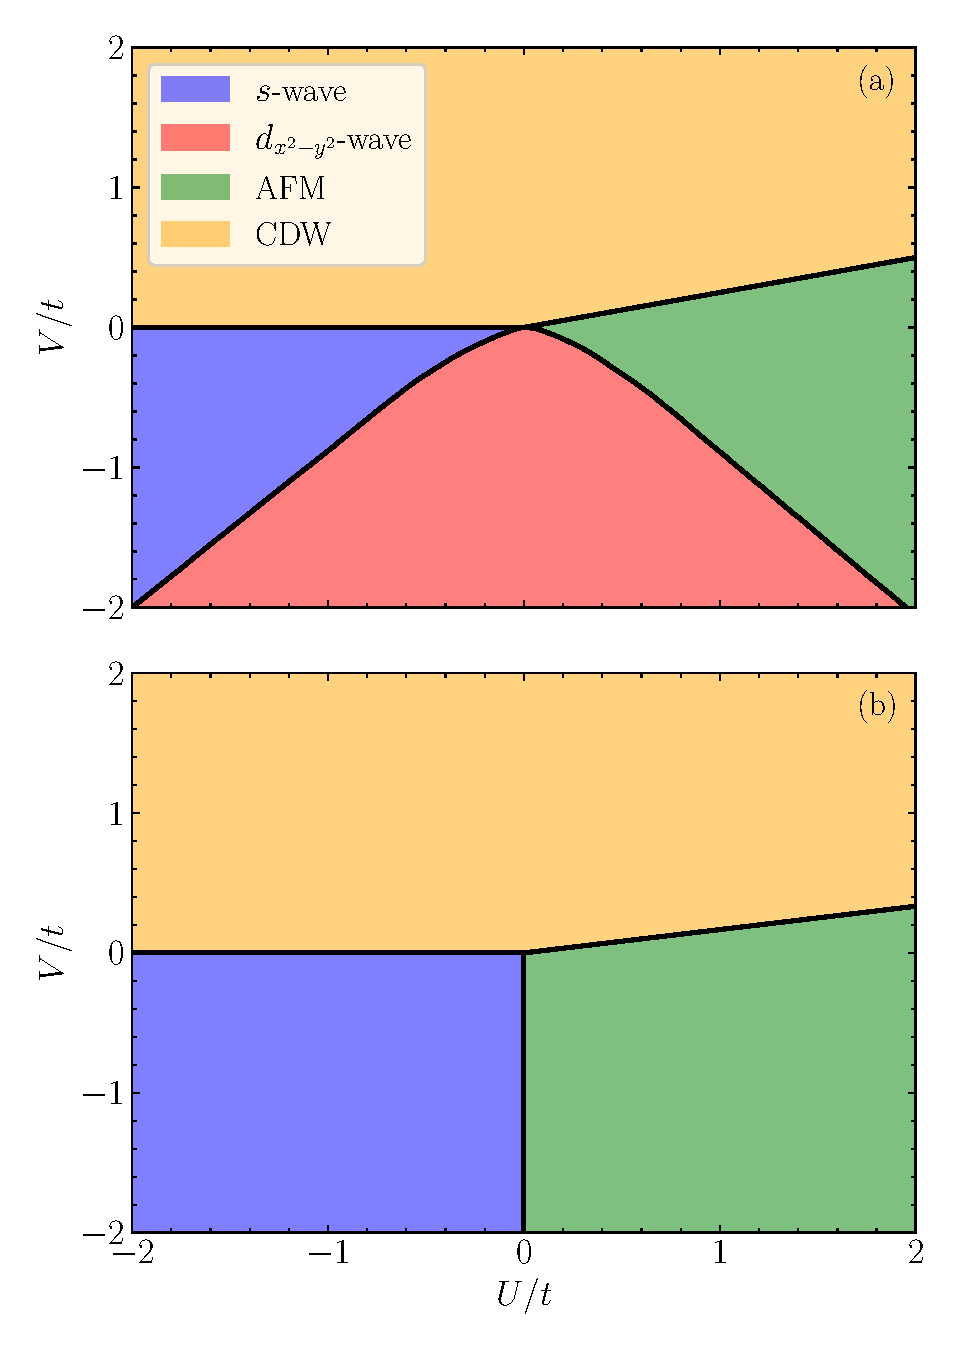
\includegraphics[width=.48\textwidth]{plots/phase_diagram.pdf}
    \caption{The phase diagram obtained for the extended Hubbard model on 
    (a) a square lattice and (b) a simple cubic lattice using a mean-field approximation at temperature $T=0$.
    The CDW-AFM boundary lies at $U = zV$, where $z$ is the coordination number. 
    For $U<0$ and $V=0$, there is a coexistence of CDW and $s$-wave SC.
    The boundary for the $d_{x^2 - y^2}$-wave SC (dashed line) for the square lattice has been taken from Ref. \cite{Micnas88b}, 
    as it is not accessible using our formalism.}
    \label{fig:phase_diagram}
\end{figure}

\begin{figure}
    \centering
    \includegraphics[width=.48\textwidth]{plots/phase_limits.pdf}
    \caption{The lower left corner ($U<0$ and $V<0$) of the phase diagram obtained for the extended Hubbard model on 
    (a) a square lattice and (b) a simple cubic lattice using a mean-field approximation at temperature $T=0$.
    The blue shading indicates the region where the $s$-wave superconducting phase is the proper ground state of the system.
    The green shading shows the region that we cannot access because the discretization $N_\gamma$, which is required to accurately describe the system, is too large.
    Lastly, the orange shading shows the region in which the dynamical matrix $\mM$ has negative eigenvalues, indicating that there are phases not captured by our methods.}
    \label{fig:phase_limits}
\end{figure}

We observe that the entire Hamiltonian and thus all expectation values only depend on
\begin{equation}
    \hat{\gamma}(\vk) \coloneqq \frac{1}{D} \sum_{\alpha=1}^D \cos(k_\alpha)\,,
\end{equation}
i.e., for any operator $\hat{O}$ the following relation holds 
\begin{equation}
    \label{eqn:equal_expecs}
    \langle \hat{O}_{\vk} \rangle = \langle \hat{O}_{\vk'} \rangle \eqqcolon \langle \hat{O}( \gamma ) \rangle\,,
\end{equation}
if $\hat{\gamma}(\vk) = \hat{\gamma}(\vk')$.
While two-dimensional systems around the size of $100\times100$ lattice sites can still be solved by using momentum sums,
computing solutions for large three-dimensional systems becomes impossible due to the $N=L^3$ scaling.
This issue can be resolved by using the aforementioned fact and replacing the momentum sums with energy integrals using the bare density of states (DOS)
\begin{equation}
    \rho(\gamma) \coloneqq  \frac{1}{N} \sum_{\vk} \delta \left(\gamma - \hat{\gamma} (\vk) \right)\,.
\end{equation}
As an example, we consider 
\begin{equation}
    \Delta_\text{SC} = \frac{U}{N} \int_{-1}^{1} \dgamma \rho(\gamma) \langle f( \gamma ) \rangle\,.
\end{equation}
We will be using the exact densities of states for the square and the simple cubic lattice found in Ref. \cite{Hanisch97}.
This allows us to access both two- and three-dimensional models on equal footing.
We can compute any phase as long as it does not introduce another kind of momentum dependence.

We solve the mean-field equations self-consistently.
The $\gamma$-integrals are approximated numerically using a $\tanh$-$\sinh$ quadrature \cite{takahasi73}, 
terminating once $|1 - \int \dgamma \rho(\gamma)| < 10^{-13}$ and reusing the computed points and weights.
This method excels at dealing with the singularities in the DOS, 
requiring merely a few hundred function evaluations to achieve the desired accuracy.

This procedure yields the ground state phase diagram at temperature $T=0$ shown in \autoref{fig:phase_diagram}.
The CDW-AFM boundary is located at $U = zV$, where $z$ is the coordination.
This holds for both the square lattice ($z=4$) and the simple cubic lattice ($z=6$) and can be seen by comparing \eqref{eqn:delta_cdw} and \eqref{eqn:delta_afm}:
Crossing the aforementioned line, changes which prefactor of the two order parameters is larger.

Note, that the $d_{x^2 - y^2}$-superconducting state, which has been confirmed for the square lattice \cite{Micnas88b,Huang13}, cannot be described by our method. 
This is due to our restriction to terms that are proportional to $\hat{\gamma}(\vk)$.

%%%%%%%%%%%%%%%%%%%%%%%%%%%%%%%%%%%%%%%%%%%%%%%%%%%%%%%%%%%%%%%%%%%%%%%%%%%%%%%%%%%%%%%%%%%%%%%%%%%%%%%%%%%%%%%%%%%%%
%%%%%%%%%%%%%%%%%%%%%%%%%%%%%%%%%%%%%%%%%%%%%%%%%%%%%%%%%%%%%%%%%%%%%%%%%%%%%%%%%%%%%%%%%%%%%%%%%%%%%%%%%%%%%%%%%%%%%
%%%%%                                                  Methods                                                  %%%%%
%%%%%%%%%%%%%%%%%%%%%%%%%%%%%%%%%%%%%%%%%%%%%%%%%%%%%%%%%%%%%%%%%%%%%%%%%%%%%%%%%%%%%%%%%%%%%%%%%%%%%%%%%%%%%%%%%%%%%
%%%%%%%%%%%%%%%%%%%%%%%%%%%%%%%%%%%%%%%%%%%%%%%%%%%%%%%%%%%%%%%%%%%%%%%%%%%%%%%%%%%%%%%%%%%%%%%%%%%%%%%%%%%%%%%%%%%%%

\section{Iterated equations of motion and Green's functions}\label{sec:ieom}

So far we have discussed the static mean-field equations that essentially describe the static ground state.
These results will be used to compute the quantities, namely expectation values, necessary for the iterated equations of motion approach \cite{uhrig09,hamerla13,hamerla14,bleicker18}.
With it, we can describe two-particle quantities like the various collective excitations of the system.

We start with some operator set $\mathcal{B}$ that is complete with respect to commutation with a Hamiltonian $H$, 
i.e., any commutator $[H, A]$ for any $A \in \mathcal{B}$ can be represented by linear combinations of operators in $\mathcal{B}$.
We can then express any time-dependent operator from this set as
\begin{equation}
    a(t) = \sum_j c_j(t) A_j\,,
\end{equation}
where $c_j(t)$ captures the entire time dependence. 
Inserting this into the Heisenberg equation of motion and applying an operator scalar product $(A_i|\cdot)$ to both sides of the equation yields
\begin{equation}
    \label{eqn:heisenberg}
    \begin{aligned}
        \ddt a(t) = \sum_j \ddt c_j(t) A_j &= i \sum_j c_j(t) [H, A_j] \\
        \Rightarrow \sum_j \underbrace{(A_i | A_j)}_{\coloneqq \mN_{ij}} \ddt c_j(t) &= i \sum_j \underbrace{(A_i | [H, A_j])}_{\coloneqq \mM_{ij}} c_j(t) \\
        \Rightarrow \mN \ddt \vec{c}(t) &= i \mM \vec{c}(t)\,.
    \end{aligned}
\end{equation}
The matrices $\mN$ and $\mM$ contain all the dynamics and energetic properties of the system.
The former is referred to as a dynamical matrix while the latter is called a norm matrix.
The advantage is that one can now handle simple matrices rather than operators acting on an enormous Hilbert space.
The size of these matrices depends entirely on the set of operators.

The matrix $\mM$ is positive semidefinite if the system is in thermal equilibrium.
We prove this statement in the appendix \autoref{sec:positive_M}.
We can use this fact to further enhance our ground state phase diagram.
If $\mM$ has even a single negative eigenvalue for any combination of parameters, we know that the system is not in thermal equilibrium, 
i.e., our self-consistency did not capture the correct ground state phase.
This does in fact happen for certain $U<0$ and $V<0$, see the orange shading in \autoref{fig:phase_limits}.
For finite temperatures, on a square lattice, a phase-separated state as well as the coexistence of a phase-separated state with $s$-wave superconductivity has been found in this region \cite{Linner23}.
The phase boundary that we propose here is qualitatively in good agreement with the one found in the aforementioned reference.
We expect a similar set of phases to be present on the simple cubic lattice but cannot prove this statement at this point.

Additionally, note that while the existence of a negative eigenvalue of $\mM$ proves that the system is not in thermal equilibrium, the absence of one does not prove the contrary.
For example, we do not find any negative eigenvalues of $\mM$ in the $U>0$, $V<0$ region despite previous studies finding $d_{x^2 - y^2}$-wave superconductivity there \cite{Micnas88b,Huang13}.

However, most Hamiltonians do not allow any such operator set to exist as the commutation usually introduces terms of higher order.
For instance, commuting a bilinear term with a quartic Hamiltonian yields, quartic terms. Repeating the commutation yields hexartic ones and so on.
Therefore, one repeats this commutation process and includes the occurring terms within a bigger set,
hoping to get better results as the set size increases.

In this article, we will be using the operator pseudo scalar product
\begin{equation}
\label{eqn:scalar_product}
    (A | B) \coloneqq  \langle [A^\dagger, B] \rangle\,,
\end{equation}
where the expectation values are taken with respect to the thermal equilibrium of the mean-field Hamiltonian \eqref{eqn:mf_hamiltonian}.
Note, that this is not a proper scalar product, as a norm defined using it can also be negative.
For example, assume that for some operator $A$
\begin{equation}
    ||A|| = (A | A) = \langle [A^\dagger, A] \rangle > 0\,,
\end{equation}
then
\begin{equation}
    ||A^\dagger|| = (A^\dagger | A^\dagger) = \langle [A, A^\dagger] \rangle = - ||A|| < 0\,.
\end{equation}
Nevertheless, this does not pose any issue in our calculations.
We will compute $\mM$ by commutating with the full Hubbard Hamiltonian \eqref{eqn:full_hamiltonian} enabling us to capture collective behavior rather than the one particle dynamics given by the mean-field approximation.

We create our operator set on the basis of \eqref{eqn:equal_expecs}.
It consists of operators of the type
\begin{equation}
    \label{eqn:ieom_basis_operator}
    A_\gamma \coloneqq \frac{1}{\sqrt{N}} \sum_{\vk} \delta (\gamma - \hat{\gamma}( \vk )) A_{\vk}\,,
\end{equation}
where $A_{\vk}$ represents each type of operator in \eqref{eqn:operators} and their Hermitian conjugates.
Operators with different indices are put into the set individually, e.g., $n_{\gamma \up}$, and $n_{\gamma \down}$ are distinct operators in our set.

Naturally, we have to discretize $\gamma$, 
however, this allows us to obtain good results with drastically smaller matrices compared to a momentum-based operator set and obtain results for a three-dimensional system in the first place.
Practically, we choose $N_\gamma = 3000$ equally spaced discretization points.
A detailed explanation of the numerics is provided in the appendix \autoref{sec:numerical_ieom}.
Herein lies the computational restriction of our method.
If the gap $\Delta_\text{tot}$ is of the same order of magnitude as our discretization $\Delta \gamma$ our numerics become inaccurate.
This manifests specifically whenever a spectral function has strong features at minuscule energies, e.g., the phase mode in the superconducting phase.
In this case, the dynamical matrix $\mM$ picks up negative eigenvalues that vanish if $N_\gamma$ is increased so that $\Delta \gamma$ is sufficiently smaller than $\Delta_\text{tot}$.

Next, we order these operators in a way reminiscent of the $x$- and $p$-terms in the harmonic oscillator, i.e.,
\begin{equation}
    X_i \coloneqq  A_i + A_i^\dagger\,,\quad P_i \coloneqq  A_i - A_i^\dagger\,.
\end{equation}
Then, our set is given by $\mathcal{B}_{XP} \coloneqq \{ X_i, \ldots, P_i, \ldots \}$.
If some operators would be 0 ($P_i$ for any $n$-type term) or duplicates (certain $X_i$ for $g$-type terms), we omit them.

Due to this choice of set, the matrices occurring in \eqref{eqn:heisenberg} have a special block structure
\begin{equation}
    \label{eqn:xp_set}
    \mM = \begin{pmatrix}
        \mathcal{K}_+ & \kappa \\ \kappa^\dagger & \mathcal{K}_-
    \end{pmatrix}\,,\quad \mN = \begin{pmatrix}
        \Lambda_+ & \mathcal{L} \\ \mathcal{L}^\dagger & \Lambda_-
    \end{pmatrix}\,,
\end{equation}
where the upper block refers to all $X_i$ and the lower block to all $P_i$.
Furthermore, due to symmetry, the relations $\Im [\mathcal{K}_\pm] = \Re [\kappa] = 0$ and $\Re [\Lambda_\pm] = \Im [\mathcal{L}] = 0$ hold.
Thus, if all occurring expectation values are real, both matrices have large empty blocks.
This condition is fulfilled for all cases investigated in this article.

To study the collective excitations, we investigate various retarded Green's functions 
\begin{equation}
    G_{AB}^\text{ret} (t) = - i \langle [A(t), B] \rangle \Theta(t)\,,
\end{equation}
and their Fourier-transformed
\begin{equation}
    \label{eqn:standard_gf}
    G_{AB}(z = \omega + i0^+) = -i \int_0^{\infty} e^{izt} \langle [A(t), B] \rangle \mathrm{d}t\,,
\end{equation}
where $\Theta(t)$ is the Heaviside function.
Our previous choice of pseudo scalar product enables us to write down a matrix-valued Green's functions in terms of the aforementioned matrices
\begin{align}
    \label{eqn:green_function}
    \mathcal{G}(z &= \omega + i0^+) = \mN \frac{1}{-z \mN - \mM} \mN \\
        &\coloneqq  -\mN \mathcal{R}(z) \mN\,,
\end{align}
where we used the resolvent
\begin{equation}
    \label{eqn:resolvent}
    \mathcal{R}(z) \coloneqq  \frac{1}{z \mN + \mM}\,.
\end{equation}
The entries of this matrix $\mathcal{G}(z)$ are the Fourier-transformed Green's functions mentioned in \eqref{eqn:standard_gf} with respect to the operators from the initially chosen set.
For instance, assume the operator in the set is $f_{\vk}$, then the top left element of $\mathcal{G}$ is the Green's function 
\begin{align}
    \mathcal{G}_{00}(z = \omega +i0^+) &=  G_{f_{\vk} f_{\vk}^\dagger} (z) \nonumber \\
        &= -i \int_0^{\infty} \langle [f_{\vk}(t), f_{\vk}^\dagger(0)] \rangle e^{izt} \mathrm{d}t\,.
\end{align}

In the following, we will derive this relation.
For that, consider the Fourier-transformed Green's function \eqref{eqn:standard_gf} with respect to two operators $A$ and $B^\dagger$ that are included in our operator set
\begin{align}
    G_{AB^\dagger} (z) &= - i \int_0^\infty \exp(i z t) \langle [ A(t), B^\dagger(0) ] \rangle \mathrm{d}t
\end{align}
Since $A$ and $B$ are included in the operator set, we can rewrite them as dot products of the vector
\begin{equation}
    \vec{A} \coloneqq  \left( A_1, A_2, \dots, A_N \right)\,, \quad
    \vec{A}^\dagger \coloneqq  \begin{pmatrix}
        A_1^\dagger \\ A_2^\dagger \\ \vdots \\ A_N^\dagger
    \end{pmatrix}\,,
\end{equation}
and some other complex-valued vector $\vec{a}$ which has its coefficients set in such a way,
that $\vec{a} \cdot \vec{A}$ is equal to the desired operator. 
For instance, $\vec{a} \equiv \vec{e}_1$ in order to represent $A_1$.

Furthermore, assuming, that $\mN$ is invertible, we can easily solve the differential equation \eqref{eqn:heisenberg} to obtain
\begin{equation}
    \vec{c}(t) = \exp \left( i \mN^{-1} \mM t \right) \vec{c}(0)\,.
\end{equation}
This allows us to finally obtain
\begin{align}
    \label{eqn:green_derivation}
    G_{AB^\dagger} (z) &= i \int_0^\infty \exp(izt) \langle [ (\vec{A \cdot} \vec{b}(0))^\dagger, \vec{A} \cdot \vec{a}(t) ] \rangle\ \mathrm{d}t \nonumber \\
        &= i \int_0^\infty \exp(izt) \vec{b}^\dagger(0) \underbrace{\langle [ \vec{A}^\dagger, \vec{A} ] \rangle}_{\equiv \mN} \vec{a}(t) \mathrm{d}t \nonumber \\
        &= i  \int_0^\infty \vec{b}^\dagger(0) \mN \exp \left( i \left(\mN^{-1} \mM + z \right) t \right) \vec{a}(0) \mathrm{d}t  \nonumber \\
        &= - \vec{b}^\dagger(0) \left[ \mN \frac{1}{\mN^{-1} \mM + z} \right] \vec{a}(0) \nonumber \\
        &= - \vec{b}^\dagger(0) \left[ \mN \frac{1}{ \underbrace{\mM + z \mN}}_{\equiv \mathcal{R}(z)} \mN \right] \vec{a}(0)\,,
\end{align}
where $\vec{a}(0)$ and $\vec{b}(0)$ are chosen such, that their product with $\vec{A}$ yields $A(0)$ and $B(0)$, respectively.
The task at hand is finding the resolvent as $\mathcal{R}$.

To do that, we embrace this matrix structure in \eqref{eqn:xp_set} and assume that all matrix entries are real.
Then, with $\mathcal{R}|_X$ denoting the block of a matrix $\mathcal{R}$ corresponding to the $X$-operators, we can calculate
\begin{align}
    r_X (z) &\coloneqq \mathcal{R}(z)|_X = \left. \frac{1}{\mM + z \mN} \right\vert_X \nonumber \\
        &= \left[ \frac{1}{\mM} - \frac{1}{\mM} z \mN \frac{1}{\mM} + \frac{1}{\mM} z \mN \frac{1}{\mM} z \mN \frac{1}{\mM} - \cdots \right]_X \nonumber \\
        &= \left. \frac{1}{\mM} \sum_{j=0}^\infty \left( -z \mN \frac{1}{\mM} \right)^j \right\vert_X \,.
\end{align}
We may omit every second element of the sum, as we want to obtain the upper left block of the matrix, and $\mN$ always swaps the upper left and lower right block.
Thus, we obtain
\begin{align}
    r_X (z) &= \left. \frac{1}{\mM} \sum_{j=0}^\infty z^{2j} \left( \mN \frac{1}{\mM} \right)^{2j} \right\vert_X \nonumber \\
        &= \left. \frac{1}{\mM - z^2 \mN \mM^{-1} \mN} \right\vert_X \nonumber \\
        &= \frac{1}{\mathcal{K}_+ - z^2 \mathcal{L} \mathcal{K}_-^{-1} \mathcal{L}^\dagger}\,.
\end{align}
Next, we define $\check{N} \coloneqq \mathcal{L} \mathcal{K}_-^{-1} \mathcal{L}^\dagger$ for brevity.
Since $\mathcal{M}$ is positive semidefinite and block diagonal, its blocks $\mathcal{K}_\pm$ must be positive semidefinite as well.
Therefore, $\check{N}$ is also positive semidefinite and we can define its square root.
We obtain
\begin{equation}
    r_X (z) = -\check{N}^{-1/2} \frac{1}{z^2 - \check{N}^{-1/2} \mathcal{K}_+ \check{N}^{-1/2}} \check{N}^{-1/2}\,.
\end{equation}
The matrix $\check{M} \coloneqq \check{N}^{-1/2} \mathcal{K}_+ \check{N}^{-1/2}$ is positive semidefinite and Hermitian by the previous arguments.
If $\check{N}$ has a singular part, the inverse can be replaced by the pseudo-inverse.
The same calculation can be repeated by exchanging $X$ with $P$, yielding the relation for the remaining block.
Then, the definitions of the matrices above change in the following way
\begin{equation}
    \check{N}_P \coloneqq \mathcal{L}^\dagger \mathcal{K}_+^{-1} \mathcal{L}\,,\quad \check{M}_P \coloneqq \check{N}_P^{-1/2} \mathcal{K}_- \check{N}_P^{-1/2}\,.
\end{equation}
In conclusion, the Green's function is given by
\begin{subequations}
    \begin{align}
        G_{AB^\dagger} \vert_P (z) &= - \left[ \vec{b}^\dagger (0) \right]_P \mathcal{L}^\dagger r_X (z) \mathcal{L} \left[ \vec{a}(0) \right]_P\,, \\
        G_{AB^\dagger} \vert_X (z) &= - \left[ \vec{b}^\dagger (0) \right]_X \mathcal{L} r_P (z) \mathcal{L}^\dagger \left[ \vec{a}(0) \right]_X\,.
    \end{align}
\end{subequations}

%%%%%%%%%%%%%%%%%%%%%%%%%%%%%%%%%%%%%%%%%%%%%%%%%%%%%%%%%%%%%%%%%%%%%%%%%%%%%%%%%%%%%%%%%%%%%%%%%%%%%%%%%%%%%%%%%%%%%
%%%%%                                                  Figures                                                  %%%%%
%%%%%%%%%%%%%%%%%%%%%%%%%%%%%%%%%%%%%%%%%%%%%%%%%%%%%%%%%%%%%%%%%%%%%%%%%%%%%%%%%%%%%%%%%%%%%%%%%%%%%%%%%%%%%%%%%%%%%

\begin{figure*}
    \centering
    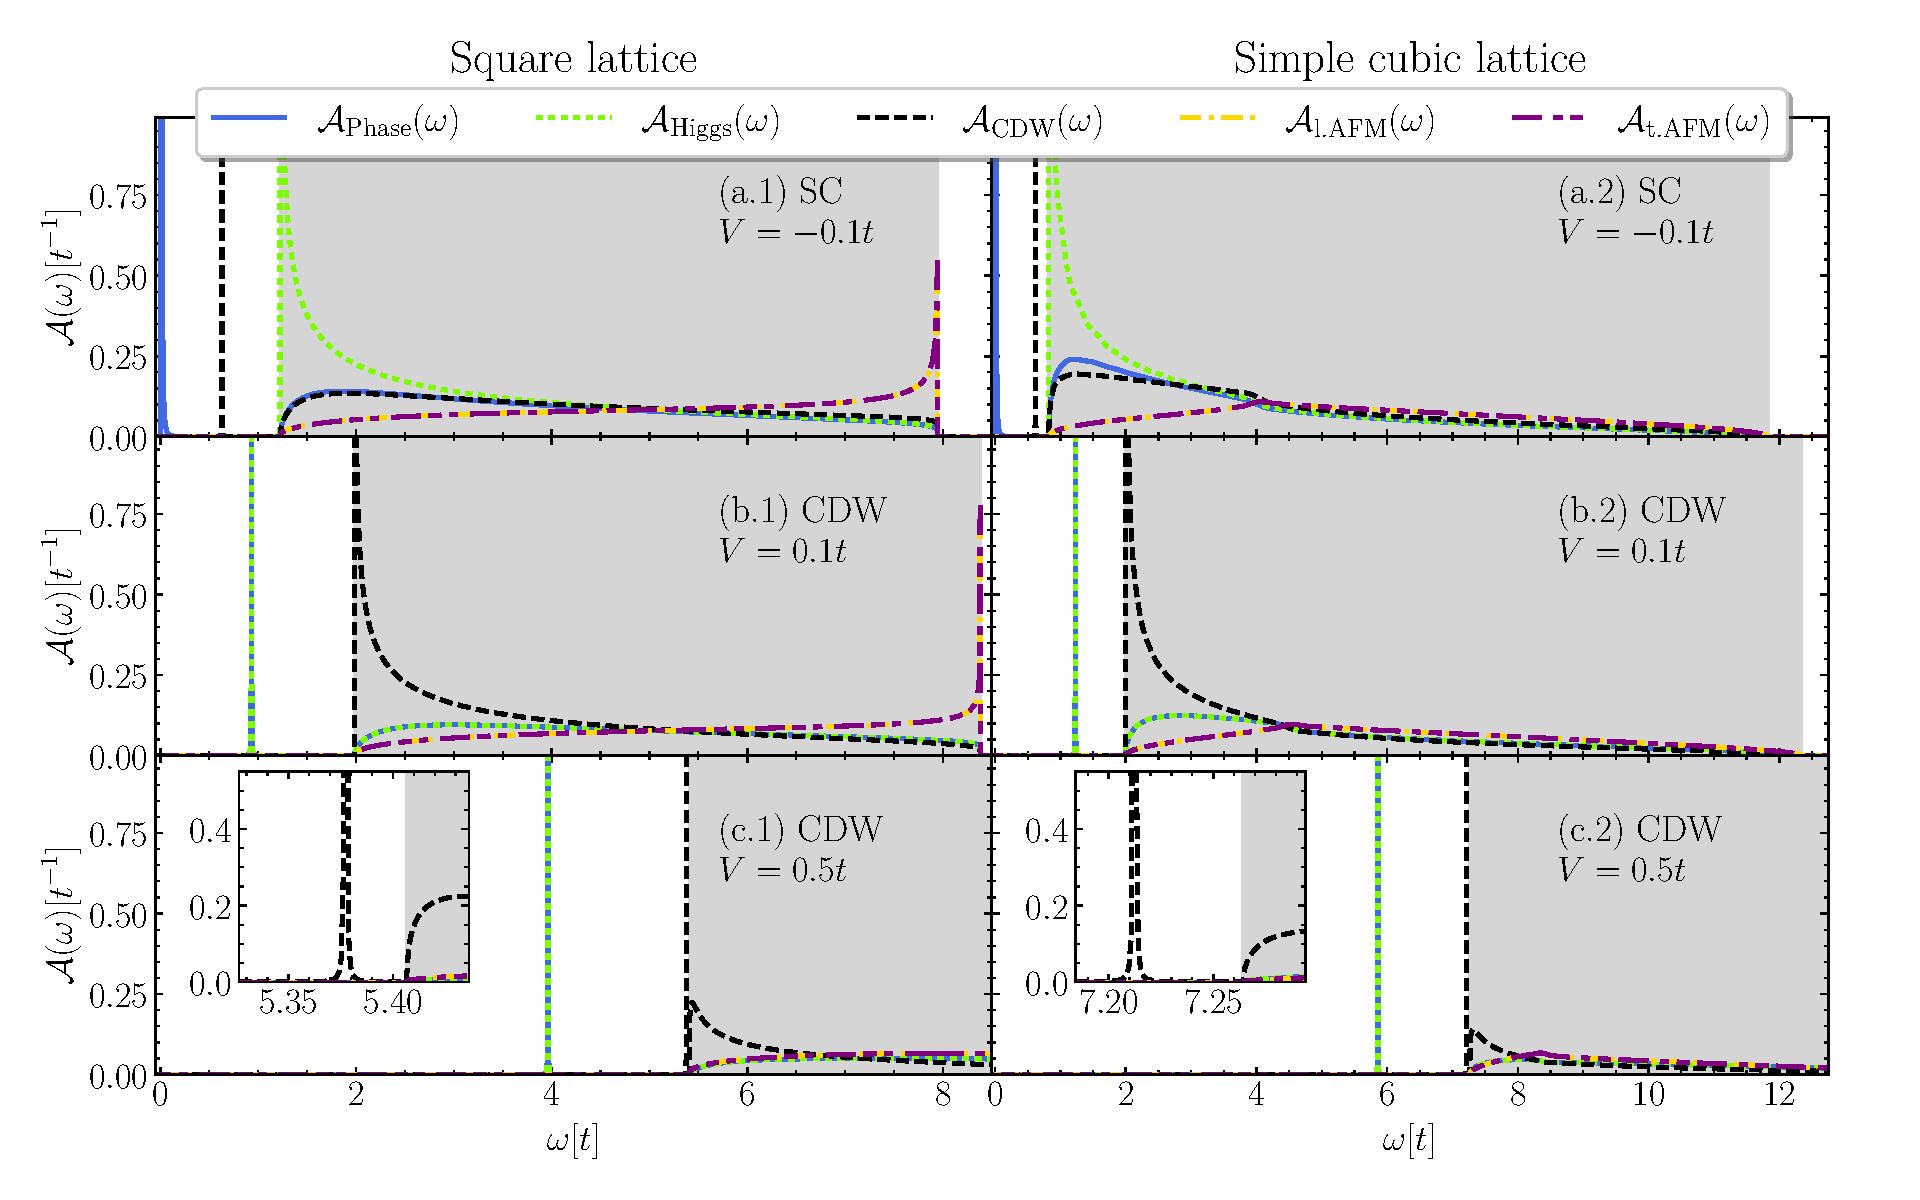
\includegraphics[width=.98\textwidth]{plots/resolvent_overview_SC_CDW.pdf}
    \caption{Spectral functions with respect to the operators listed in \eqref{eqn:resolvent_bases}.
    The left column shows the results for the square lattice while the right column shows the results for the simple cubic lattice.
    The left edge of each plot is at $-0.05$ rather than $0$ in order to improve the visibility of the phase peak.
    The shaded area marks the two-particle continuum.
    For each plot, the parameters are set to $U=-2.5t$ and $N_\gamma = 3000$, while $V$ is varied according to the text in the individual panels.
    The panels show the spectral functions in the (a) SC phase and the (b and c) CDW phase, respectively.}
    \label{fig:resolvent_overview_SC}
\end{figure*}

\begin{figure*}
    \centering
    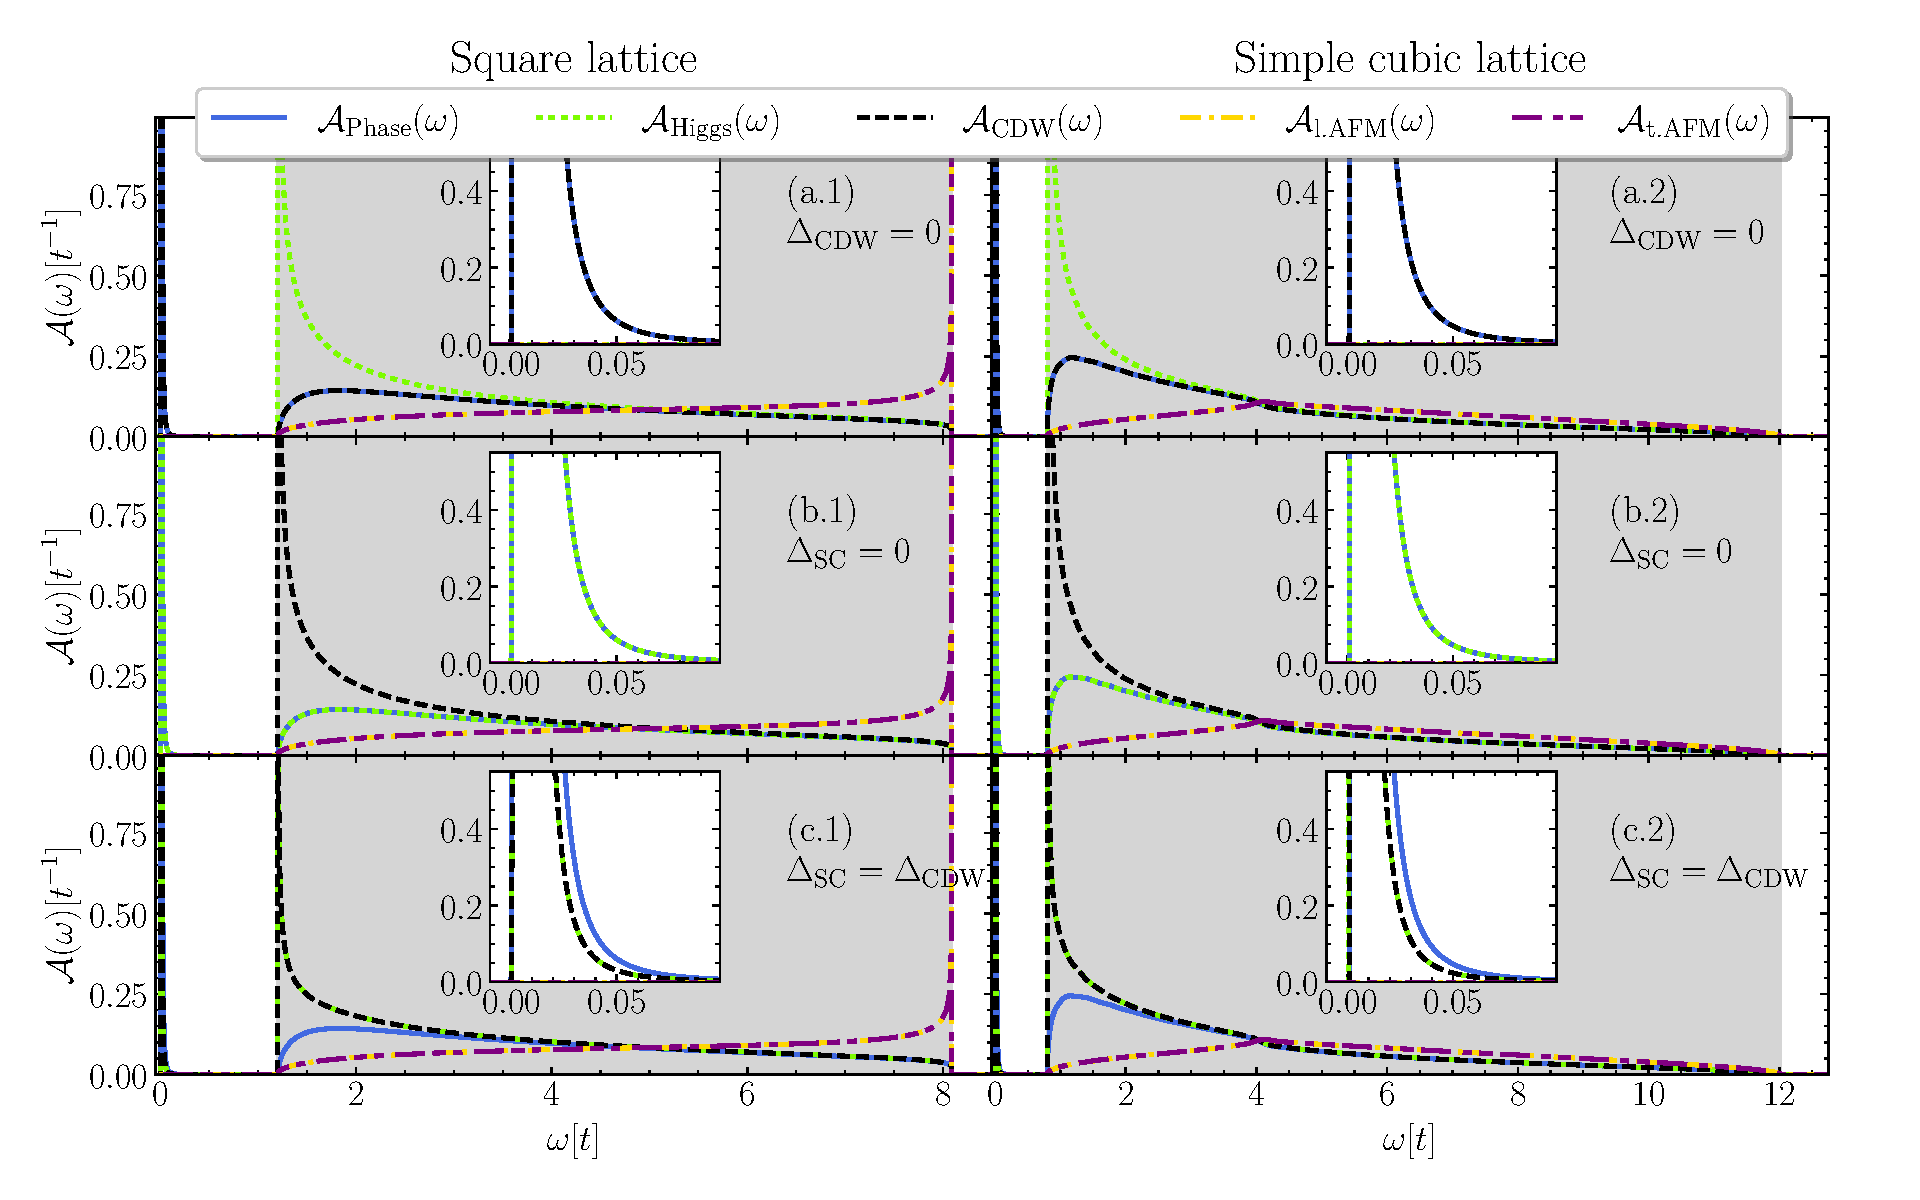
\includegraphics[width=.98\textwidth]{plots/resolvent_overview_V0.pdf}
    \caption{Spectral functions with respect to the operators listed in \eqref{eqn:resolvent_bases}.
    The left column shows the results for the square lattice while the right column shows the results for the simple cubic lattice.
    The left edge of each plot is at $-0.05$ rather than $0$ in order to improve the visibility of the peaks at $\omega=0$.
    The shaded area marks the two-particle continuum.
    For each plot, the parameters are set to $U=-2.5t$, $V=0$, and $N_\gamma = 3000$.
    Since the ratio of $\Delta_\text{SC}$ to $\Delta_\text{CDW}$ may be chosen arbitrarily, we show in (a) the spectral functions for $\Delta_\text{CDW} = 0$ and in (b) for $\Delta_\text{SC} = 0$.}
    \label{fig:resolvent_overview_V0}
\end{figure*}

\begin{figure*}
    \centering
    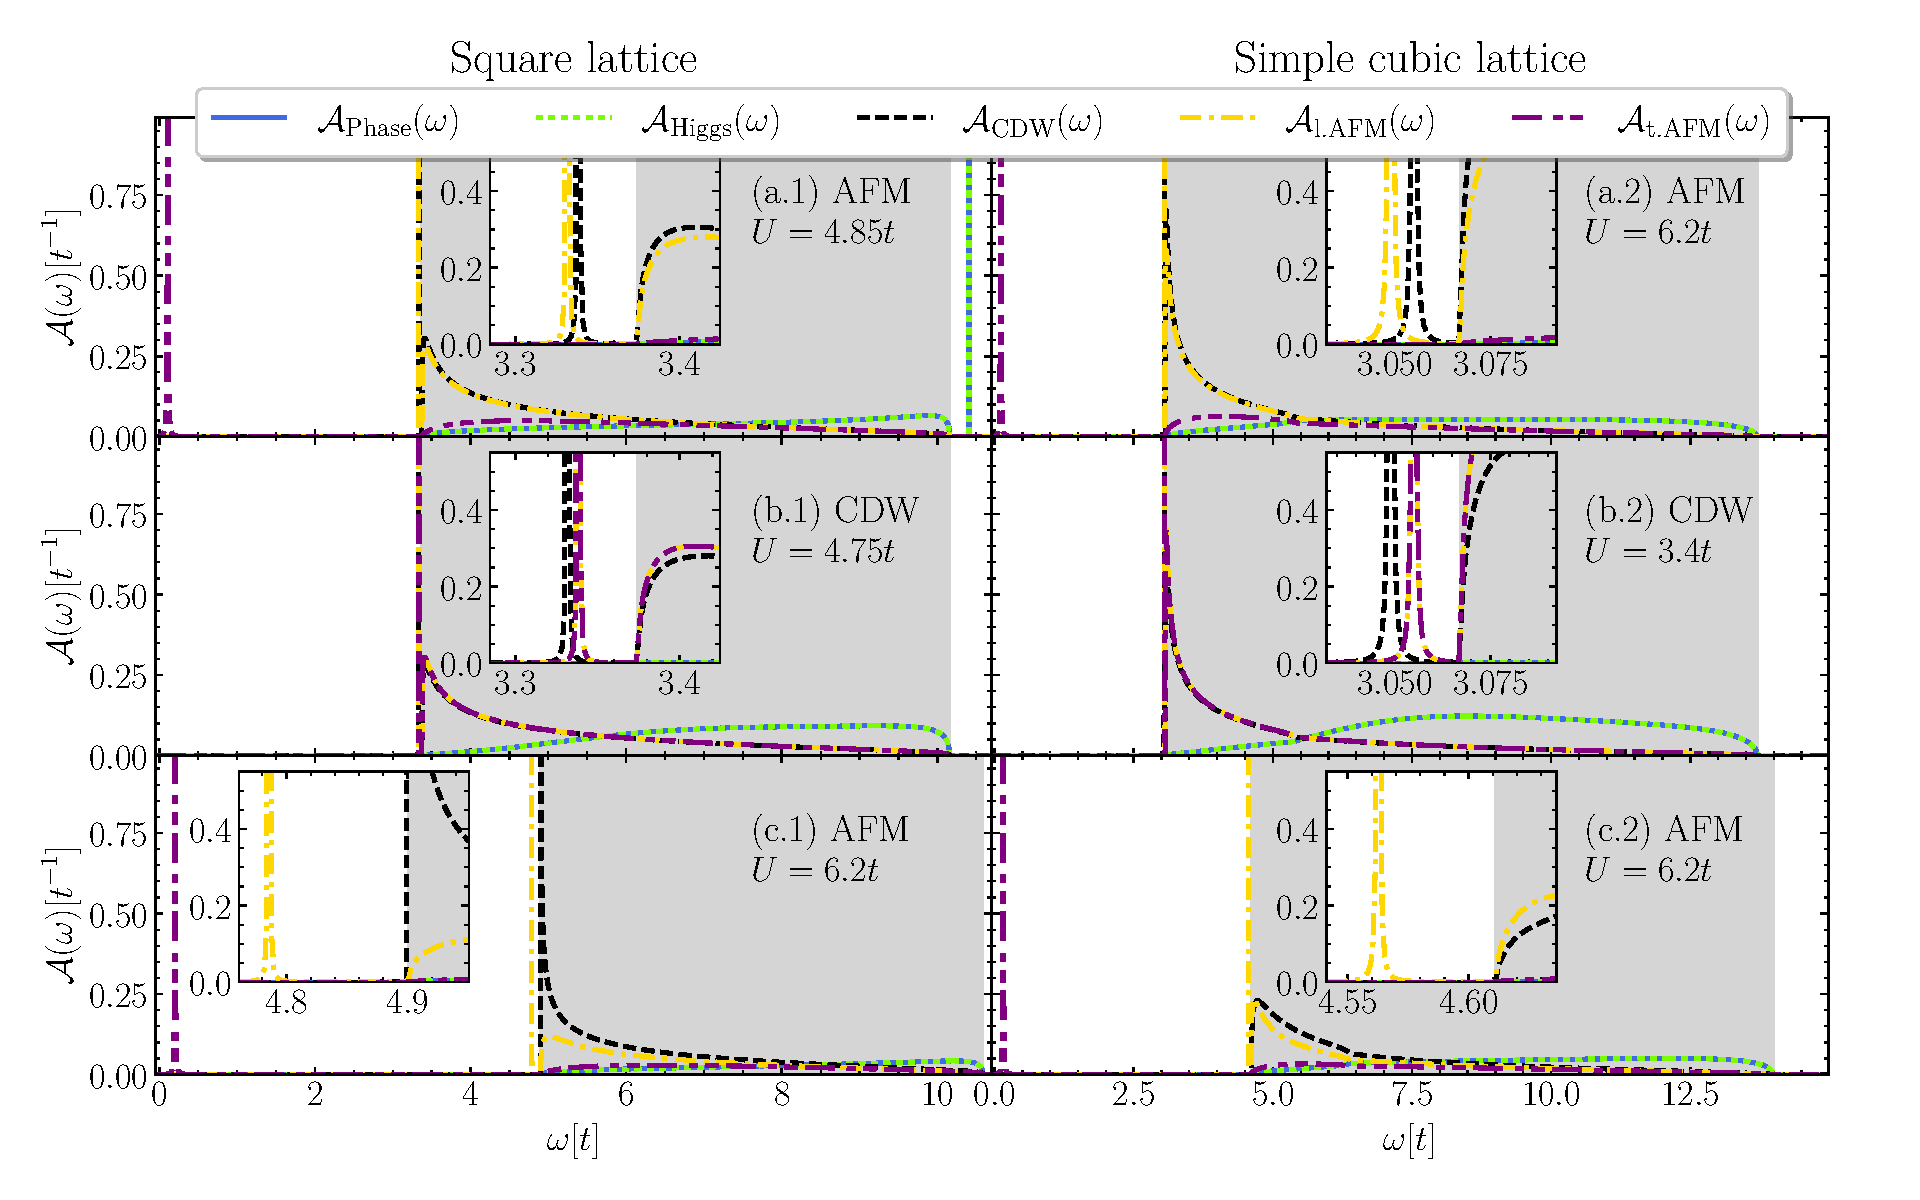
\includegraphics[width=.98\textwidth]{plots/resolvent_overview_AFM_CDW.pdf}
    \caption{Spectral functions with respect to the operators listed in \eqref{eqn:resolvent_bases}.
    The left column shows the results for the square lattice while the right column shows the results for the simple cubic lattice.
    The shaded area marks the two-particle continuum.
    For each plot, the parameters are set to $V=1t$ and $N_\gamma = 3000$, while $U$ is varied according to the text in the individual panels.
    The panels (a) and (c) show the spectral functions in the AFM phase, and the panels (b) and (d) in the CDW phase.}
    \label{fig:resolvent_overview_AFM}
\end{figure*}

\begin{figure*}
    \centering
    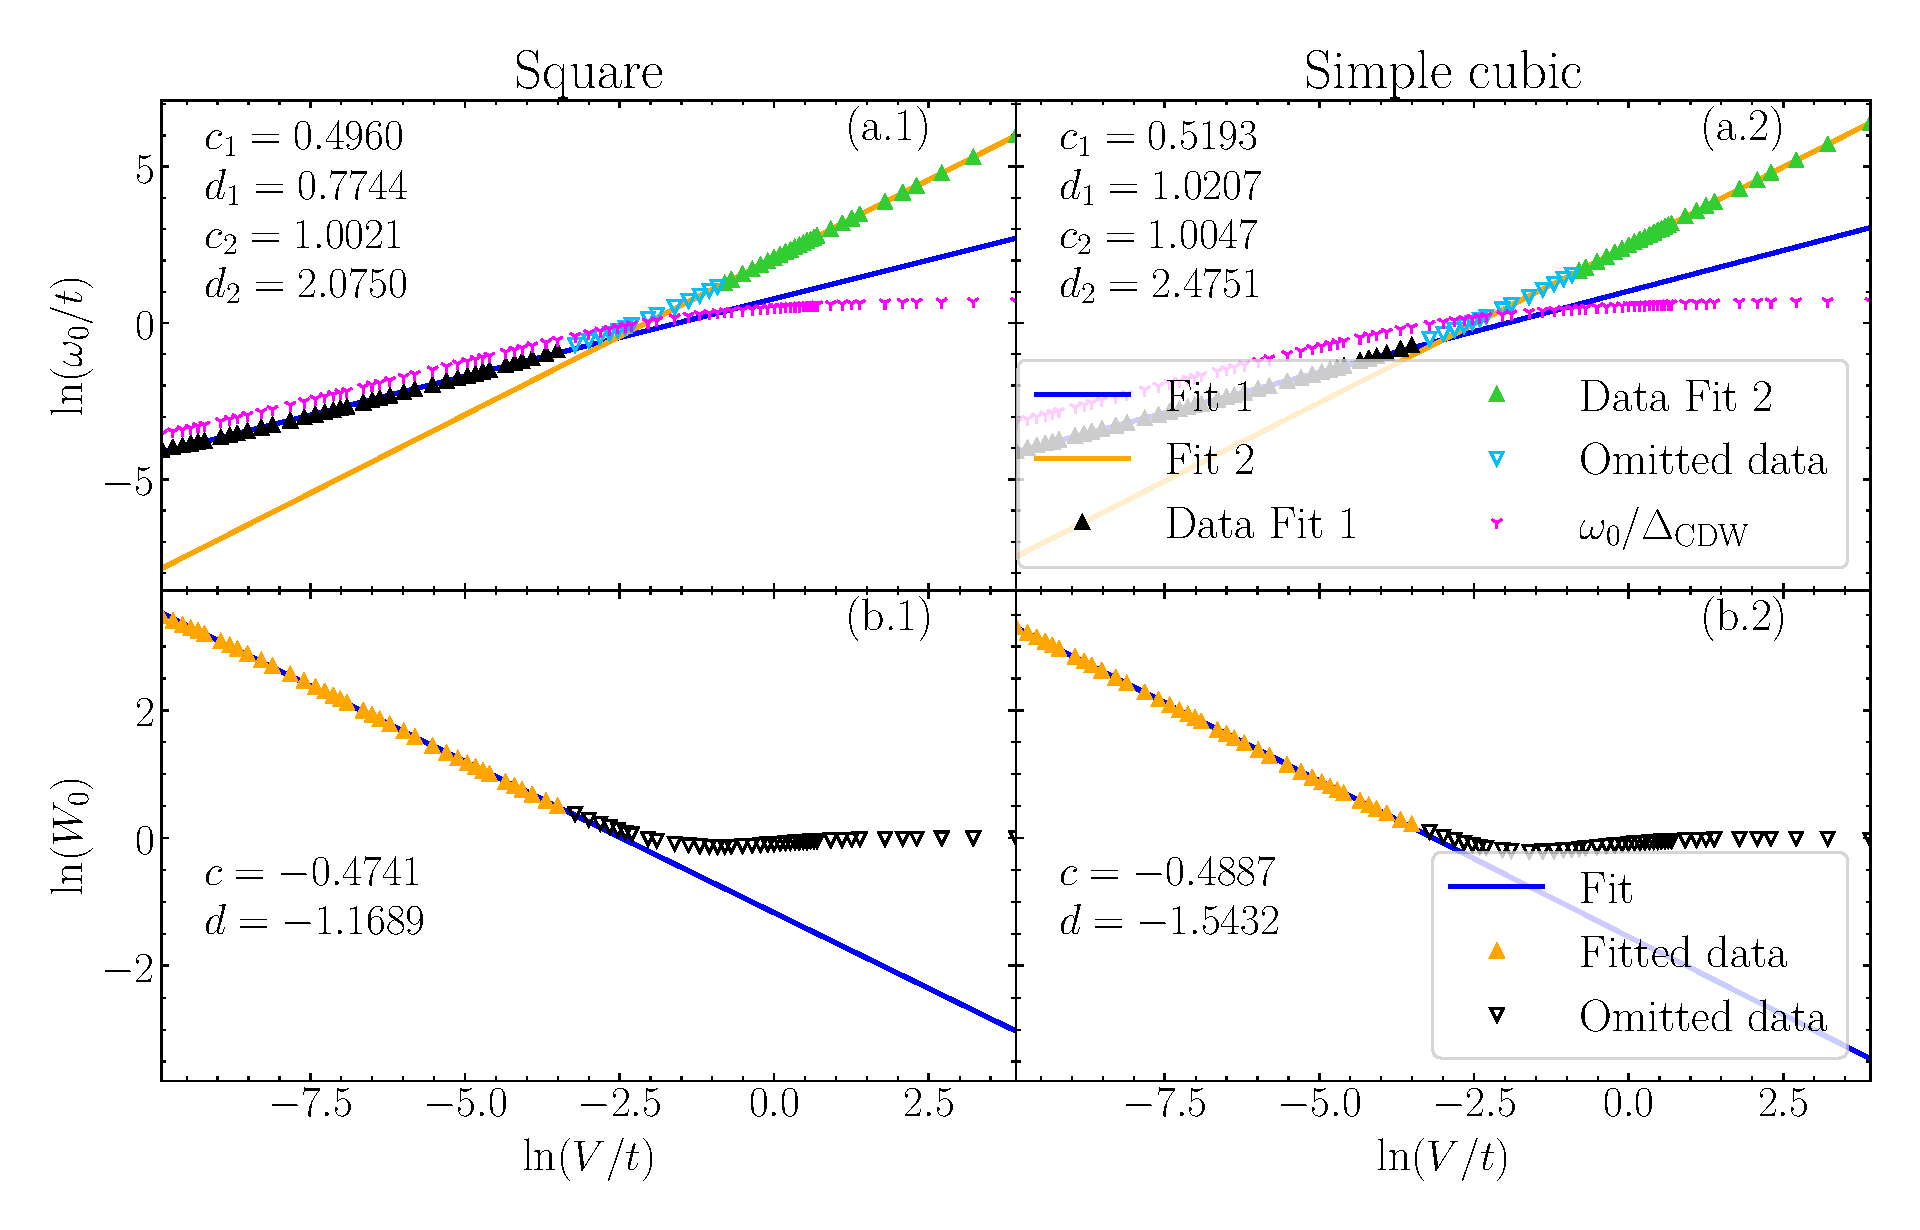
\includegraphics[width=.98\textwidth]{plots/sc_peak_in_cdw.pdf}
    \caption{The upper panels (a) show double logarithmic plots of the positions $\omega_0$ of the peak in $\spectral{SC}$ in the CDW phase while the lower panels (b) show their respective weights $W_0 = e^{b}$.
    In the upper panels, the pink markers additionally show the peak position divided by the gap $\omega_0 / \Delta_\text{CDW}$.
    The left column shows the results for the square and the right column for the simple cubic lattice at $U=-2.5t$.
    The fits are linear, i.e., $y(V) = c \ln(V/t) + d$, and the parameters are printed on the individual panels.}
    \label{fig:sc_in_cdw_behavior}
\end{figure*}

\begin{figure*}
    \centering
    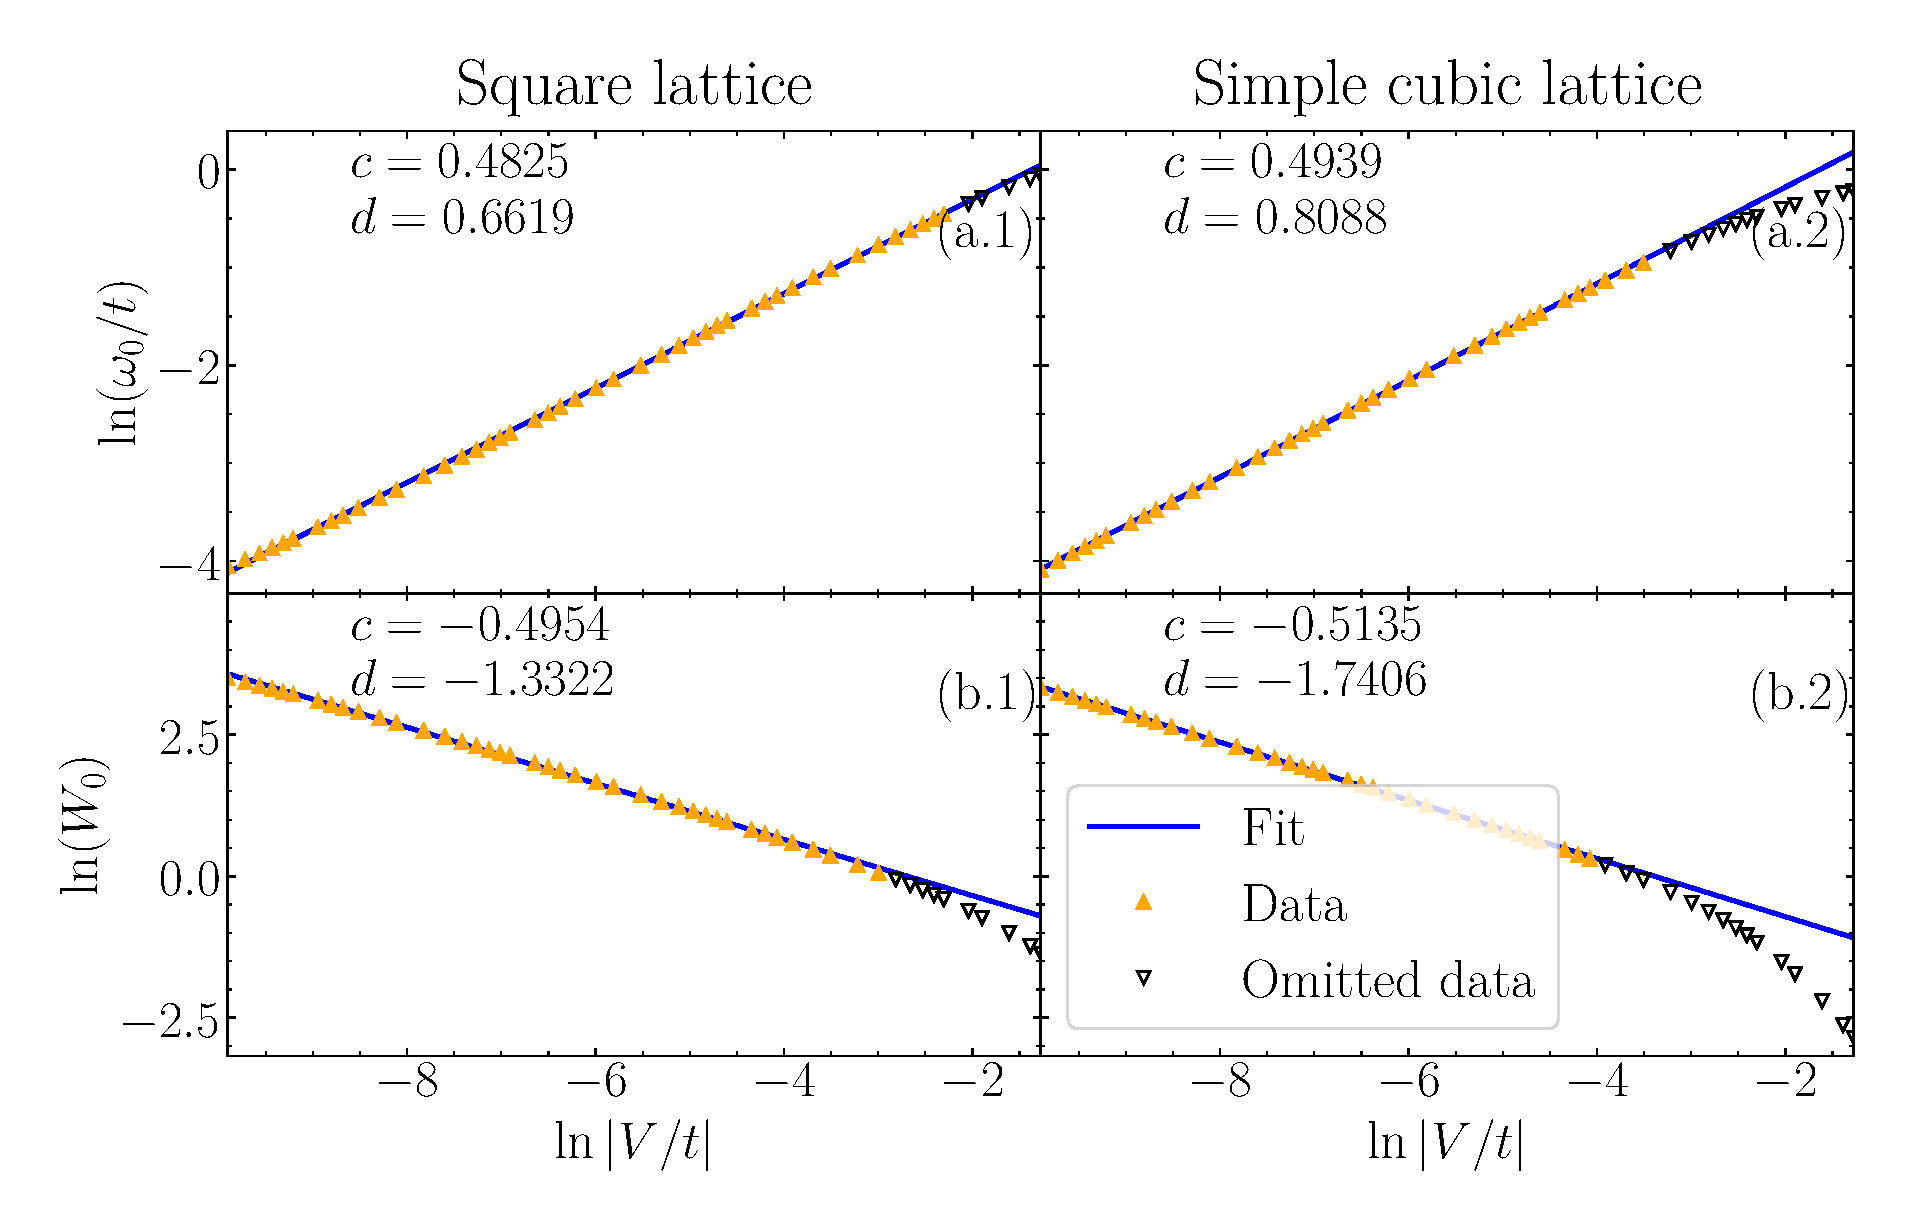
\includegraphics[width=.98\textwidth]{plots/cdw_peak_in_sc.pdf}
    \caption{The panels (a) show plots of the positions $\omega_0$ of the peak in $\spectral{CDW}$ in the SC phase.
    Below that, in panels (b), their respective weights are depicted.
    The dashed lines in both rows show the position or weight computed for $V=0$ with $\Delta_\text{CDW} = 0$.
    The left column shows the results for the square and the right column for the simple cubic lattice at $U=-2.5t$.
    The left-most values are $V=-0.28t$ for the square lattice and $V=-0.34t$ for the simple cubic lattice.
    Choosing even smaller values results in $\mathcal{M}$ no longer being positive, i.e., the system is not in thermal equilibrium.
    \newline
    The lower panels (c) and (d) present the data again, but with logarithmic scaling on the $V$-axis.
    Additionally, the peak positions and weights are given relative to their value at $V=0$.
    These data are fitted by $y(x) = a (\tanh (bx - c) + 1)$ with the parameters printed in the individual panel.
    The panels (a) and (b) feature the same fitting result.}
    \label{fig:cdw_in_sc_behavior}
\end{figure*}

\begin{figure*}
    \centering
    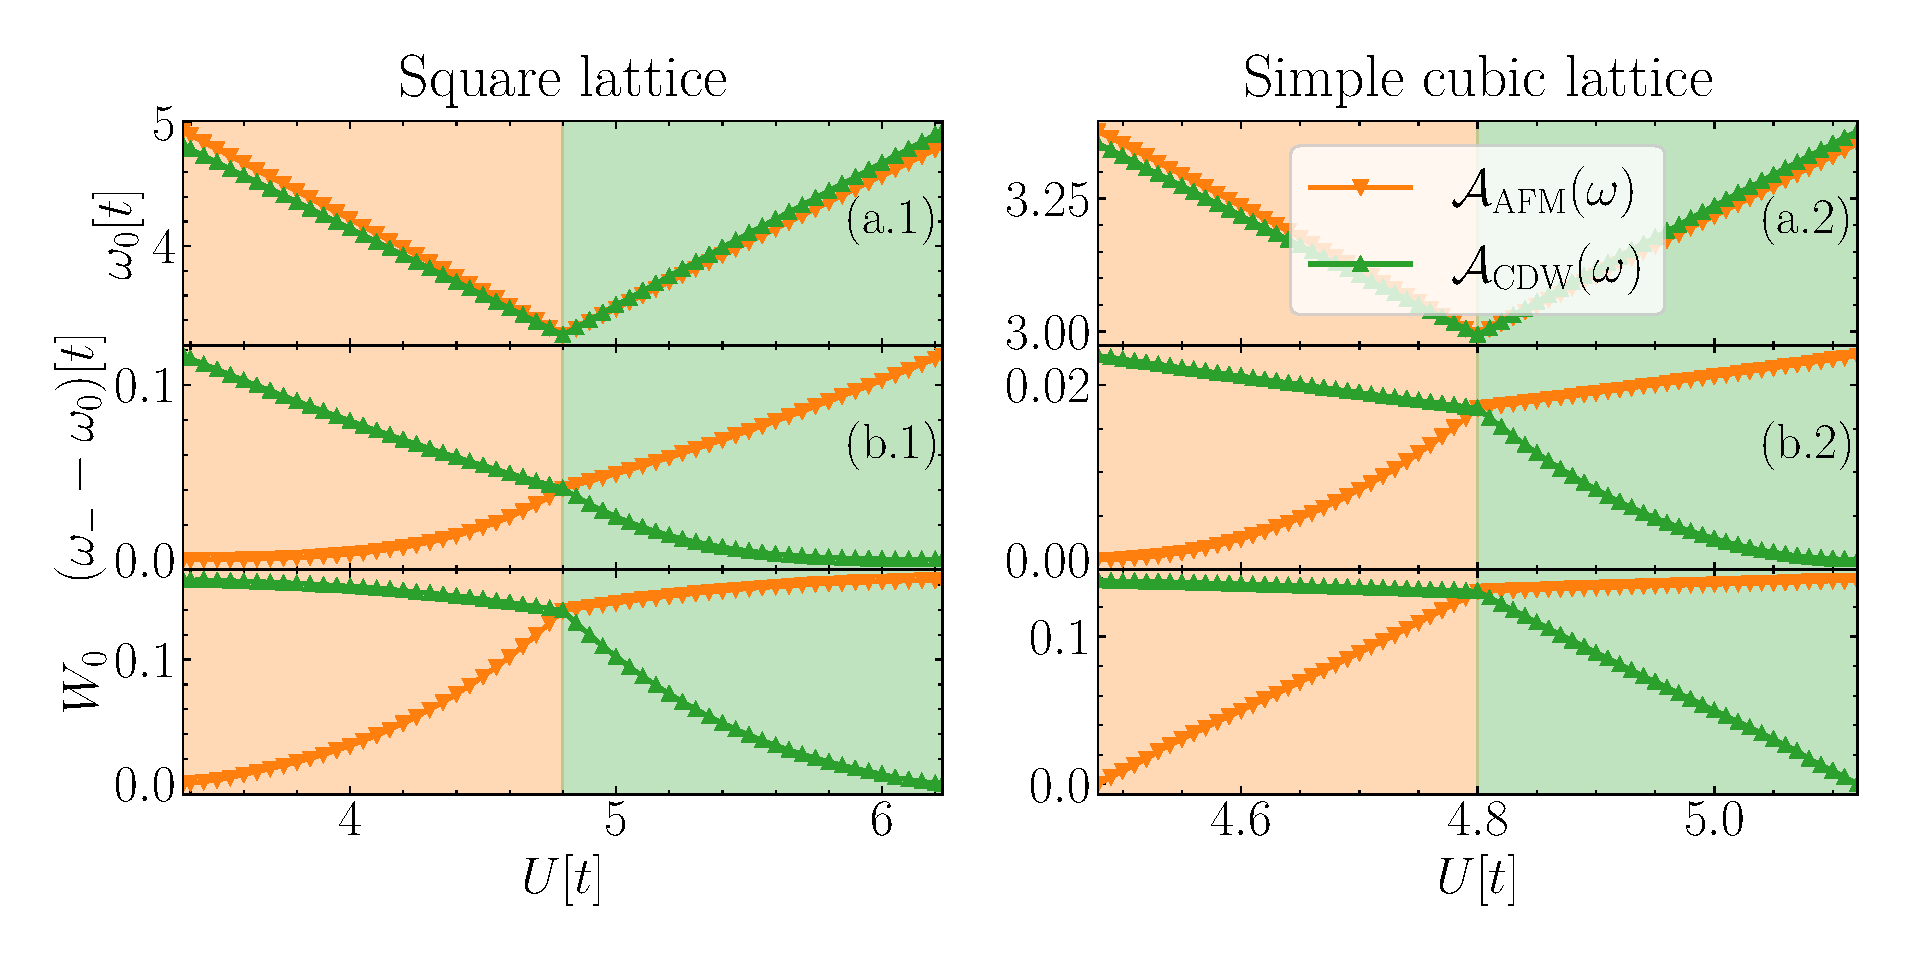
\includegraphics[width=.98\textwidth]{plots/afm_cdw_peaks_overview.pdf}
    \caption{The upper panels (a) show plots of the positions $\omega_0$ of the peak in $\spectral{CDW}$ (orange lines) and $\spectral{AFM}$ (blue lines) close to the corresponding phase transition $U = zV$.
    The middle panels (b) depict the peak positions relative to the lower edge of the two-particle continuum $\omega_-$, while the bottom panels (c) show their respective weights.
    The shadings indicate the phase the system is in. Blue represents AFM while orange represents CDW.
    The left column shows the results for the square and the right column for the simple cubic lattice at $V=-1t$.
    Note the difference in the scales for the two lattices.}
    \label{fig:afm_cdw_peaks_overview}
\end{figure*}

\begin{figure*}
    \centering
    \includegraphics[width=.98\textwidth]{plots/afm_cdw_peaks_details.pdf}
    \caption{The upper panels (a) show plots of the positions $\omega_0$ of the peak in $\spectral{AFM}$ relative to the lower edge of the two-particle continuum $\omega_-$.
    The lower panels (b) depict their respective weights $W_0$.
    The left column shows the results for the square and the right column for the simple cubic lattice at $V=-1t$.
    $U_0$ denotes the highest value of $U$ for which there is no peak below the two-particle continuum.
    For the square lattice it is $U_0 = 3.5775t$ and for the simple cubic lattice it is $U_0 = 4.89t$.
    The parameter range depicted here places the system within the CDW phase.
    All fits are linear, i.e., $y=ax + b$.}
    \label{fig:afm_cdw_peaks_details}
\end{figure*}

%%%%%%%%%%%%%%%%%%%%%%%%%%%%%%%%%%%%%%%%%%%%%%%%%%%%%%%%%%%%%%%%%%%%%%%%%%%%%%%%%%%%%%%%%%%%%%%%%%%%%%%%%%%%%%%%%%%%%
%%%%%                                                  Figures                                                  %%%%%
%%%%%%%%%%%%%%%%%%%%%%%%%%%%%%%%%%%%%%%%%%%%%%%%%%%%%%%%%%%%%%%%%%%%%%%%%%%%%%%%%%%%%%%%%%%%%%%%%%%%%%%%%%%%%%%%%%%%%

Now, the task at hand is finding the inverse $1/(z^2 - \check{M})$ for all $z$.
This can be achieved using a Lanczos tridiagonalization and subsequently a continued fraction expansion in the form of

\begin{widetext}
\begin{equation}
    \left( z^2 - \begin{pmatrix}
        a_0 & b_1 & 0 & 0 & \cdots \\
        b_1 & a_1 & b_2 & 0 & \cdots \\
        0 & b_2 & a_2 & b_3 & \cdots \\
        0 & 0 & b_3 & a_3 & \cdots \\
        \vdots & \vdots & \vdots & \vdots & \ddots
    \end{pmatrix} \right)_{00}^{-1} = \dfrac{1}{z^2 - a_0 - \dfrac{b_1^2}{z^2 - a_1 - \dfrac{b_2^2}{ z^2 - a_2 - \hdots}}}\,\,
\end{equation}
\end{widetext}

where $a_i$ and $b_i$ are the Lanczos coefficients \cite{PettiforRecursion,ViswanathRecursion}.

Obtaining a diagonal block of $\mathcal{G}$ is easily achieved by setting $\vec{b}(0) = \vec{a}(0)$.
Obtaining an off-diagonal block requires linear combinations in the form of 
\begin{align}
    \vec{a}^\dagger \mathcal{G} \vec{b} &= \frac{1}{4} \Big\{ 
        \underbrace{\left[ (\vec{a} + \vec{b})^\dagger \mathcal{G} (\vec{a} + \vec{b}) - (\vec{a} - \vec{b})^\dagger \mathcal{G} (\vec{a} - \vec{b}) \right]}_{ = 2 \vec{a}^\dagger \mathcal{G} \vec{b} + 2 \vec{b}^\dagger \mathcal{G} \vec{a}} \\
    &-i \underbrace{\left[ (\vec{a} + i \vec{b})^\dagger \mathcal{G} (\vec{a} + i \vec{b}) - (\vec{a} - i \vec{b})^\dagger \mathcal{G} (\vec{a} - i \vec{b}) \right]}_{= 2i \vec{a}^\dagger \mathcal{G} \vec{b} - 2i \vec{b}^\dagger \mathcal{G} \vec{a}} \Big\}\,, \nonumber
\end{align}
i.e., one computes the four diagonal blocks and then simply adds them as described above.

In the single-band case, the coefficients approach the limit
\begin{equation}
    \label{eqn:inf_lanczos}
    a_\infty = \frac{\omega_+ + \omega_-}{2}\text{  and  } b_\infty = \frac{\omega_+ - \omega_-}{4}\,,
\end{equation}
where $\omega_\pm$ represents the upper and lower band edge, respectively \cite{PettiforRecursion}.
This behavior allows us to terminate the continued fraction, once the coefficients have converged close enough to these values, using the so-called square root terminator
\begin{equation}
    T(\omega) = \frac{1}{2b_\infty^2} \left( \omega - a_\infty \mp \sqrt{(\omega - a_\infty)^2 - 4 b_\infty^2} \right)\,,
\end{equation}
where the negative sign is to be chosen for $\omega - a_\infty > 2b_\infty$ and $|\omega - a_\infty| < 2b_\infty$ and the positive one otherwise.
It is to be noted, that the coefficients start to drop off from this limit as more and more Lanczos iterations are performed \cite{ViswanathRecursion}.
Therefore, we terminate the continued fraction with the aforementioned terminator at the coefficient pair that has the least deviation from $a_\infty$ and $b_\infty$.

%%%%%%%%%%%%%%%%%%%%%%%%%%%%%%%%%%%%%%%%%%%%%%%%%%%%%%%%%%%%%%%%%%%%%%%%%%%%%%%%%%%%%%%%%%%%%%%%%%%%%%%%%%%%%%%%%%%%%
%%%%%%%%%%%%%%%%%%%%%%%%%%%%%%%%%%%%%%%%%%%%%%%%%%%%%%%%%%%%%%%%%%%%%%%%%%%%%%%%%%%%%%%%%%%%%%%%%%%%%%%%%%%%%%%%%%%%%
%%%%%                                                  Results                                                  %%%%%
%%%%%%%%%%%%%%%%%%%%%%%%%%%%%%%%%%%%%%%%%%%%%%%%%%%%%%%%%%%%%%%%%%%%%%%%%%%%%%%%%%%%%%%%%%%%%%%%%%%%%%%%%%%%%%%%%%%%%
%%%%%%%%%%%%%%%%%%%%%%%%%%%%%%%%%%%%%%%%%%%%%%%%%%%%%%%%%%%%%%%%%%%%%%%%%%%%%%%%%%%%%%%%%%%%%%%%%%%%%%%%%%%%%%%%%%%%%

\section{Results}\label{sec:results}

In this section, we will be investigating four different diagonal Green's functions $G_{AA^\dagger}(\omega + i0^+)$, namely with
\begin{subequations}
    \label{eqn:resolvent_bases}
    \begin{align}
        A_\text{Higgs} &= \frac{1}{\sqrt{N}} \sum_{\vk} \left( f_{\vk} + f_{\vk}^\dagger \right)  
            = \int \dgamma \left( f_{\gamma} + f_{\gamma}^\dagger \right) \,,\\
        A_\text{Phase} &= \frac{i}{\sqrt{N}} \sum_{\vk} \left( f_{\vk} - f_{\vk}^\dagger \right) = \int \dgamma \left( f_{\gamma} - f_{\gamma}^\dagger \right) \,,\\
        A_\text{CDW}   &= \frac{1}{\sqrt{N}} \sum_{\vk} \left( g_{\vk \up} + g_{\vk \down} \right) = \int \dgamma \left( g_{\gamma \up} + g_{\gamma \down} \right) \,,\\
        A_\text{AFM}   &= \frac{1}{\sqrt{N}} \sum_{\vk} \left( g_{\vk \up} - g_{\vk \down} \right) = \int \dgamma \left( g_{\gamma \up} - g_{\gamma \down} \right) \,,
    \end{align}
\end{subequations}
where $N$ is the number of lattice sites in the system. 
Each one of these operators generates a different kind of collective mode.
The first operator captures the amplitude mode of the $s$-wave superconducting state, while the second one catches the phase mode \cite{Fan22}.
The remaining two capture the collective behavior of the CDW and AFM states, respectively.
In the following, we will refer to the Green's functions generated by these operators as $\mathcal{G}_{i}(\omega) = G_{A_i A_i^\dagger}(\omega)$.

Note, that all of the aforementioned operators are Hermitian. 
This means that all spectral functions need to be completely antisymmetrical, see appendix \autoref{sec:antisymmetry_spectral}.
For this reason, we will only show the $\omega \geq 0$ in our plots. 
Additionally, we will add a small imaginary part of $10^{-5}t$ to $\omega$ in order to visualize the occurring $\delta$ peaks.

%%%%%%%%%%%%%%%%%%%%%%%%%%%%%%%%%%%%%%%%%%%%%%%%%%%%%%%%%%%%%%%%%%%%%%%%%%%%%%%%%%%%%%%%%%%%%%%%%%%%%%%%%%%%%%%%%%%%%
%%%%%                                              Classification                                               %%%%%
%%%%%%%%%%%%%%%%%%%%%%%%%%%%%%%%%%%%%%%%%%%%%%%%%%%%%%%%%%%%%%%%%%%%%%%%%%%%%%%%%%%%%%%%%%%%%%%%%%%%%%%%%%%%%%%%%%%%%

\subsection{Classification of the spectral functions}

To begin, let us describe the spectral functions $\mathcal{A}_i (\omega) = - (1/\pi) \Im [\mathcal{G}_i (\omega + i0^+)]$ with respect to the operators above in the various phases.
\autoref{fig:resolvent_overview_SC} shows them at $U = -2.5t$ in the SC ($V=-0.1t$) and CDW ($V=0.1t$ and $V=0.5t$) phase.

There are a variety of different features. The difference between the two lattices is mostly quantitative.
First and foremost, in the SC phase, see panel (a), 
there is a sharp peak located at $\omega=0$ in $\spectral{Phase}$ and a singularity in $\spectral{Higgs}$ located at $\omega=2\Delta_\text{SC}$.
We identify them with the well-known Anderson-Bogoliubov and Higgs modes in superconductors.
Note, that the former must not have any weight though, because the spectral function is perfectly antisymmetrical.
The peak itself can be found at zero energy because our model describes a neutral superfluid 
wherein there is no coupling of the phase of the order parameter to the electromagnetic potential.
Therefore, this phase may be chosen arbitrarily, and changing it requires no energy 
which ultimately allows a Goldstone mode to exist in the first place \cite{Goldstone1961,Anderson63}.

To classify the occurring peaks that lie outside the two-particle continuum, we turn towards the real part of the Green's function.
We plot it in close proximity to the peaks with a double logarithmic scale and fit the result linearly $y = ax + b$ to obtain its power-law behavior.
The real part is related to the imaginary part via the Kramers-Kronig relations.
Specifically, if the imaginary part is a $\delta$ distribution, the real part will be proportional to $1/\omega$, i.e., $a=-1$, and the peak has the weight $W_0 = \exp(b)$.
Furthermore, an exponent of $a=-2$ corresponds to the derivative of the $\delta$ distribution, i.e., $\delta'(\omega)$.
The fits themselves can be found in appendix \autoref{sec:fit_greens_functions}.

This analysis provides that the real part of $\greens{Phase}$ near $\omega=0$ behaves as $1/\omega^2$ indicating that the peak in $\spectral{Phase}$ is the derivative of a $\delta$ distribution.
The weight of such a peak is given by the integral $\int \delta'(\omega) \mathrm{d}\omega = 0$.
This confirms our previous expectation that this peak cannot have any weight.

The singularity in $\spectral{Higgs}$ behaves as $1/\sqrt{\omega - 2 \Delta_\text{SC}}$.
Previous studies on the dynamics of the order parameter found damped oscillations after a quench.
These have the frequency $\Omega = 2 \Delta_\text{SC}$ and fall off as $1/\sqrt{t}$ \cite{Yuzbashyan06}.
An inverse Fourier transform of $\spectral{Higgs}$ yields precisely the same behavior, thereby reinforcing the validity of our results.

In the CDW phase, see panels (b) and (c), both of $\spectral{Higgs}$ and $\spectral{Phase}$ become identical and form a $\delta$ peak below the two-particle continuum.
Following the Landau theory for continuous phase transitions, this is to be expected as the free energy is expanded in terms of the order parameter as
\begin{equation}
    f(\Delta_\text{SC}) \approx r |\Delta_\text{SC}|^2 + \frac{u}{2} |\Delta_\text{SC}|^4\,,
\end{equation}
with $r > 0$ and $u > 0$ if the system is outside of the superconducting phase. 
In this case, the only minimum is at $\Delta_\text{SC} = 0$. 
That means that both possible modes have to overcome the same energy to be excited at all. 

In the SC phase, $\spectral{CDW}$ features a $\delta$ peak below the continuum corresponding to the finite energy necessary to excite this kind of electronic density modulation.
For moderate-sized values of $V>0$, i.e., in the CDW phase, see panel (b) at $V=0.1t$, the aforementioned spectral function has a singularity at $\omega=2\Delta_\text{CDW}$.% that exhibits a square-root behavior.
This mode becomes hard and moves outside the two-particle continuum as $V$ is increased, see panel (c) at $V=0.5t$.

$\spectral{AFM}$ is restricted to the continuum for both phases and both lattices.
For the square lattice, however, there is a singularity located at the upper edge of the two-particle continuum.

%%%%%%%%%%%%%%%%%%%%%%%%%%%%%%%%%%%%%%%%%%%%%%%%%%%%%%%%%%%%%%%%%%%%%%%%%%%%%%%%%%%%%%%%%%%%%%%%%%%%%%%%%%%%%%%%%%%%%

At $V=0$, both the SC and the CDW orders coexist. 
In this phase, the mean-field single-particle energies are given by
\begin{equation}
    E_{\pm} = \pm \sqrt{\epsilon^2 + |\Delta_\text{CDW}|^2 + |\Delta_\text{SC}|^2}\,.
\end{equation}
This means that the proper order parameter is $\Delta_\text{tot} \coloneqq \sqrt{|\Delta_\text{CDW}|^2 + |\Delta_\text{SC}|^2}$.
Here, $\Delta_\text{CDW}$ and $\Delta_\text{SC}$ can change arbitrarily without affecting the system's energy as long as $\Delta_\text{tot}$ remains constant.
Note, that the degeneracy of both phases is exact due to the SO(4) symmetry \cite{yang90}. 

In \autoref{fig:resolvent_overview_V0}, we show the spectral functions for $U=-2.5t$ and $V=0$.
The different panels correspond to different choices for $\Delta_\text{CDW}$ and $\Delta_\text{SC}$.
First, in panel (a), we set $\Delta_\text{CDW} = 0$.
This results in a purely superconducting phase with the same features as in \autoref{fig:resolvent_overview_SC} panel (a).
The peak in $\spectral{CDW}$ moves to a very small, yet finite, $\omega$.
Within the two-particle continuum $\spectral{CDW}$ and $\spectral{Phase}$ are identical.

Secondly, panel (b) shows the spectral functions for $\Delta_\text{SC} = 0$, i.e., in a purely charge-ordered phase.
Similar to before, there is not much change compared to \autoref{fig:resolvent_overview_SC} panel (b).
The spectral functions $\spectral{Higgs}$ and $\spectral{Phase}$ are still identical, however, both exhibit a sharp peak at $\omega=0$.
This peak is described by $\delta'(\omega)$.

Lastly, we chose $\Delta_\text{CDW} = \Delta_\text{SC}$ for panel (c).
For this specific ratio of $\Delta_\text{CDW}$ and $\Delta_\text{SC}$, $\spectral{Higgs}$ and $\spectral{CDW}$ are identical.
Choosing a different ratio yields qualitatively the same results, but the peaks differ in magnitude.
Both spectral functions have a peak at $\omega = 0$, described by $\delta'(\omega)$, and a singularity at the lower edge of the two-particle continuum $\omega = 2\Delta_\text{tot}$.
Each one of the singularities behaves as $1/\sqrt{\omega - 2 \Delta_\text{tot}}$.

We associate the peak at $\omega=0$ with this shifting of order parameters, i.e., diminishing one and increasing the other while keeping $\Delta_\text{tot}$ constant.
The singularity at the lower edge of the two-particle continuum can be interpreted similarly to the Higgs mode in a pure superconductor.
It captures the change of $\Delta_\text{tot}$ by changing either one of the composing order parameters.

$\spectral{Phase}$ behaves just as it does in the pure SC phase. It has only a peak at $\omega = 0$ that can be associated with the change of the phase of $\Delta_\text{SC}$.

%%%%%%%%%%%%%%%%%%%%%%%%%%%%%%%%%%%%%%%%%%%%%%%%%%%%%%%%%%%%%%%%%%%%%%%%%%%%%%%%%%%%%%%%%%%%%%%%%%%%%%%%%%%%%%%%%%%%%

Lastly, we investigate the same spectral functions close to the AFM-CDW phase transition, depicted in \autoref{fig:resolvent_overview_AFM}.
We choose $V=1t$ for both lattices and $U=zV \pm 0.1t$, where $z$ is the coordination number, see panels (a) and (b).
Again, both SC-related spectral functions are identical in both the CDW and AFM phases.
Within the continuum their weight is shifted towards the upper edge and on the square lattice only, there is a peak above the continuum.
In the AFM phase, both $\spectral{AFM}$ and $\spectral{CDW}$ have a peak close, but yet below, the two-particle continuum.
The peak of the former is at a lower energy than the peak of the latter.
In the CDW phase, this behavior is reversed, i.e., the peak in $\spectral{CDW}$ lies lower.
Using the same analysis as before, we conclude that each of these peaks is a $\delta$ peak.
Moving further away from the phase transition, here $U=z(V+0.2t)$ in panels (c) and (d), the upper peak becomes soft as it shifts into the two-particle continuum. 


%%%%%%%%%%%%%%%%%%%%%%%%%%%%%%%%%%%%%%%%%%%%%%%%%%%%%%%%%%%%%%%%%%%%%%%%%%%%%%%%%%%%%%%%%%%%%%%%%%%%%%%%%%%%%%%%%%%%%
%%%%%                                                  SC-CDW                                                   %%%%%
%%%%%%%%%%%%%%%%%%%%%%%%%%%%%%%%%%%%%%%%%%%%%%%%%%%%%%%%%%%%%%%%%%%%%%%%%%%%%%%%%%%%%%%%%%%%%%%%%%%%%%%%%%%%%%%%%%%%%

\subsection{SC-CDW transition}

With the prevalent peaks discussed, we turn towards their behavior as the system approaches the phase transition at $V=0$ for $U=-2.5t$.
First and foremost, we investigate the peak in $\spectral{Phase}$ and $\spectral{Higgs}$ in the CDW phase.
The evolution of its position $\omega_0$ and its weight $W_0$ as $V$ is varied can be viewed double logarithmically in \autoref{fig:sc_in_cdw_behavior}.
For $V \ll t$, the position grows with the square root of $V$. This behavior then transitions to a purely linear growth for large $V$.
Dividing $\omega_0$ by the gap $\Delta_\text{CDW}$ results in a plateau for large $V$ while leaving the square root behavior at the beginning mostly unchanged.

The peak weights $W_0$ fall off as $1/\sqrt{V}$ for $V \ll t$. 
Afterward, it reaches a shallow minimum and rises slightly to reach a constant value.

Specifically, we learn that for $V \ll t$, the peak position follows $\omega_0 = \alpha \sqrt{V}$ and its weight follows $W_0 = \beta / \sqrt{V}$, 
where $\alpha$ and $\beta$ are some constants.
This allows us to write $W_0 = \beta / (\alpha \omega_0)$. 
Furthermore, we know that the spectral functions need to be perfectly antisymmetrical about $\omega = 0$, i.e., we can observe
\begin{align}
    \mathcal{A}_\text{Phase} (\omega \ll t) &= W_0 (\delta (\omega - \omega_0) - \delta (\omega + \omega_0)) \nonumber \\
        &= - \frac{2\beta}{\alpha} \frac{\delta (\omega + \omega_0) - \delta (\omega - \omega_0)}{2\omega_0} \,.
\end{align} 
Taking the limit of $V \to 0$ corresponds to the limit $\omega_0 \to 0$, i.e., leading to an expression reminiscent of symmetric derivative
\begin{equation}
    \lim_{h \to 0} \frac{f(x + h) - f(x - h)}{2h} = f'(x)\,,
\end{equation}
where the equality holds for any differentiable $f$.
Applying this to our case yields
\begin{align}
    \lim_{\omega_0 \to 0} \mathcal{A}_\text{Phase} (\omega \ll t) = - \frac{2 \beta}{\alpha} \delta'(\omega)\,.
\end{align}
This analysis reinforces our previous identification of the phase peak as $\delta' (\omega)$.

%%%%%%%%%%%%%%%%%%%%%%%%%%%%%%%%%%%%%%%%%%%%%%%%%%%%%%%%%%%%%%%%%%%%%%%%%%%%%%%%%%%%%%%%%%%%%%%%%%%%%%%%%%%%%%%%%%%%%

As a next step, we want to analyze the peak in $\spectral{CDW}$ that occurs if the system is in the SC phase ($V<0$).
A plot of its position $\omega_0$ and weight $W_0$ can be seen in \autoref{fig:sc_in_cdw_behavior}.
First and foremost, the upper panels (a) and (b) depict the peak positions and weights, respectively.
The former drops off and the latter grows as $V$ moves to 0, however, both of them smoothly approach a finite value.
It is the same, as the one that is obtained for $V=0$ while setting $\Delta_\text{CDW}$ to 0, see \autoref{fig:resolvent_overview_V0} (a).
This indicates that the peak steadily evolves to the limiting case $V=0$.

Moving towards larger $|V|$, the peaks move towards greater $\omega$, i.e., closer to the two-particle continuum.
Additionally, the weights drop off, first with increasing speed and then slowing down, see panels (c) and (d) for a logarithmic scaling.
A fit of the form $y(x) = a (\tanh (bx - c) + 1)$, with $x=\ln|V/t|$ works well for both the peak positions and weights.
Transforming back to the non-logarithmic scale yields
\begin{equation}
    y(V) = a \left( \frac{ \xi - \frac{1}{\xi} }{ \xi + \frac{1}{\xi} } \right)\,,\quad \xi \coloneqq e^{-c} |V/t|^b\,.
\end{equation}
The fit parameters are printed in the respective panels of \autoref{fig:sc_in_cdw_behavior}.
This indicates that the peak weights drop off fairly quickly as the system moves away from the phase transition while the peak positions shift towards higher energies.
It also suggests that there might be a finite saturation value, but we are unable to compute the Green's functions for additional, even larger $|V|$, 
because the matrix $\mM$ is not nonnegative anymore after $V\approx -0.28t$ (square lattice) or $V\approx -0.34t$ (simple cubic lattice).
Note, that our proof for the nonnegativity is based on the system being in thermal equilibrium.
Therefore, we conclude that beyond these values of $V$, the superconducting phase is not the true ground state of the system, see \autoref{fig:phase_limits}.
Specifically, the $s$-wave superconducting phase on the square lattice seems to be even smaller than first estimated using the $d_{x^2 -y^2}$ data from \cite{Micnas88b}.
In recent research, there has been evidence for a phase-separated state for negative values of $V$ on a square lattice, which would explain our results here \cite{Linner23}.
It would be reasonable to assume, that this phase occurs in both the 2- and 3-dimensional case.
The magnitude of $V$ for which our calculation stops working is in the same order as in the referenced paper.
Note, however, that we did our computations at $T=0$ while the reference worked on finite temperature systems.


%%%%%%%%%%%%%%%%%%%%%%%%%%%%%%%%%%%%%%%%%%%%%%%%%%%%%%%%%%%%%%%%%%%%%%%%%%%%%%%%%%%%%%%%%%%%%%%%%%%%%%%%%%%%%%%%%%%%%
%%%%%                                                  AFM-CDW                                                  %%%%%
%%%%%%%%%%%%%%%%%%%%%%%%%%%%%%%%%%%%%%%%%%%%%%%%%%%%%%%%%%%%%%%%%%%%%%%%%%%%%%%%%%%%%%%%%%%%%%%%%%%%%%%%%%%%%%%%%%%%%

\subsection{AFM-CDW transition}

Lastly, we investigate how the modes behave as the system transitions between the CDW and AFM phases.
Similar to the previous subsection, we plot the occurring peaks in $\spectral{CDW}$ and $\spectral{AFM}$ within the respective phase in \autoref{fig:afm_cdw_peaks_overview}.
On the right side of each panel, i.e., for $U > zV$, the system is in the AFM phase (blue shading).
On the left side, it is in the CDW phase (orange shading).
In general, the peak in $\spectral{AFM}$ behaves exactly as the peak in $\spectral{CDW}$ if the phases are swapped.

The panel (a) shows the peak positions unmodified. They essentially move linearly as $U$ is varied.
It is noteworthy, that in the AFM phase, the peak in $\spectral{AFM}$ lies lower than the one in $\spectral{CDW}$.
Naturally, this is reversed, if the system is in the CDW phase.
This is to be expected, as creating an AFM excitation should be energetically more favorable if the system is already in said phase.

Additionally, we plot in (b) the peak positions relative to the lower edge of the two-particle continuum.
We see that the lower-lying peak, i.e., the peak corresponding to the phase the system is in, 
strays further away from the continuum as the system moves away from the phase boundary.
The other peak, however, moves ever closer to the aforementioned continuum until they reach it.
At this point, the weight of said peak also vanishes, see panel (c).
This occurs around $U \approx 4V \pm 0.4245t$ for the square lattice and around $U \approx 6V \pm 1.11t$ for the simple cubic lattice.

On the square lattice, the weights of the peaks in $\spectral{AFM}$ in the AFM phase (the same applies to $\spectral{CDW}$ in the CDW phase) grow as the system moves away from the phase transition.
On the simple cubic lattice, however, the weights fall off very slightly.

In \autoref{fig:afm_cdw_peaks_details}, we revisit panels (b) and (c) from the previous figure.
We restrict the analysis to $\spectral{AFM}$ in the CDW phase as the reverse case yields precisely the same data.
This time around the scaling is double-logarithmic and we consider $U$ relative to those values at which we cannot find a peak in $\spectral{AFM}$.
This occurs around $U_0 = 3.5755t$ on the square lattice and around $U_0 = 4.89t$ on the simple cubic lattice.
This yields that the peak positions $\omega_0$ (a) behave quadratically as they move into the two-particle continuum,
while their weights $W_0$ (b) drop off linearly.

%%%%%%%%%%%%%%%%%%%%%%%%%%%%%%%%%%%%%%%%%%%%%%%%%%%%%%%%%%%%%%%%%%%%%%%%%%%%%%%%%%%%%%%%%%%%%%%%%%%%%%%%%%%%%%%%%%%%%
%%%%%%%%%%%%%%%%%%%%%%%%%%%%%%%%%%%%%%%%%%%%%%%%%%%%%%%%%%%%%%%%%%%%%%%%%%%%%%%%%%%%%%%%%%%%%%%%%%%%%%%%%%%%%%%%%%%%%
%%%%%                                                Conclusion                                                 %%%%%
%%%%%%%%%%%%%%%%%%%%%%%%%%%%%%%%%%%%%%%%%%%%%%%%%%%%%%%%%%%%%%%%%%%%%%%%%%%%%%%%%%%%%%%%%%%%%%%%%%%%%%%%%%%%%%%%%%%%%
%%%%%%%%%%%%%%%%%%%%%%%%%%%%%%%%%%%%%%%%%%%%%%%%%%%%%%%%%%%%%%%%%%%%%%%%%%%%%%%%%%%%%%%%%%%%%%%%%%%%%%%%%%%%%%%%%%%%%

\section{Conclusion}\label{sec:conclusion}


We have conducted an analysis of the mean-field phase diagram of the extended Hubbard model in 2D and 3D. 
Specifically, both systems provide a similar structure of $s$-wave SC, CDW, and AFM.
Furthermore, we were able to identify an area in which our analysis is incomplete.
In 2D, this region coincides with a phase-separated state that has already been observed in recent research \cite{Linner23}.

We have also developed a novel method to obtain Fourier transformed Green's functions and analyzed various such functions. 
We have found collective excitations within the spectral functions $\spectral{Higgs}$, $\spectral{Phase}$, $\spectral{CDW}$, and $\spectral{AFM}$ 
and examined their behavior as the system approaches phase transitions. 
In particular, we identified the peak and singularity found in the first two as the well-known phase and amplitude modes in neutral superconductors 
and thereby provided a technique to obtain them starting from a microscopic description.

We observed the behavior of the peak in the SC-related spectral functions.
It moves towards 0 energy and attains more weight as the system moves from the CDW phase towards the SC phase. 
The peak's relative position to the two-particle continuum and its weight plateau as the system moves away from the phase transition.

In the SC phase close to the CDW phase, the peak in $\spectral{CDW}$ is located at a finite energy and and has a finite weight. 
It moves towards higher energy and its weight drops off as the system moves away from the phase transition. 

Around the AFM-CDW phase transition, both $\spectral{AFM}$ and $\spectral{CDW}$ feature a peak. 
The peak of the former in the AFM phase lies at lower energies than the latter one and vice-versa. 
Moving away from the phase transition, the higher-lying peak becomes soft as it moves into the two-particle continuum. 
The peak position relative to the two-particle continuum approaches $0$ quadratically with $U$, and its weight approaches $0$ linearly.

Furthermore, we have found a peak in $\spectral{CDW}$ that appears at large values of $V$, 
which is most likely the same as the one found close to the CDW-AFM phase transition. 

%%%%%%%%%%%%%%%%%%%%%%%%%%%%%%%%%%%%%%%%%%%%%%%%%%%%%%%%%%%%%%%%%%%%%%%%%%%%%%%%%%%%%%%%%%%%%%%%%%%%%%%%%%%%%%%%%%%%%

Some possible ideas for future research include incorporating phase-separated states into the mean-field theory.
This would enable us to peer deeper into the negative $V$ regime of the phase diagrams and provide more analysis of the collective excitations that occur therein.

Moreover, one can fathom to include a coupling of the electronic system to the electromagnetic field.
This should move the position of the phase mode close to the plasma frequency as explained by the Anderson-Higgs mechanism.

Additionally, one could describe multi-band systems with even richer phases and collective excitations. 


%==============================================================================
% Acknowledgments 
%==============================================================================
\begin{acknowledgments} 
    ....
\end{acknowledgments}

\appendix
\section{Semipositivity of the dynamical matrix}
\label{sec:positive_M}

We show that $\mathcal{M}$ is positive semidefinite if the system is in thermal equilibrium.
For any $\vec{x} \in \mathbb{C}^N$, consider
\begin{align}
    \vec{x}^\dagger \mM \vec{x} &= \sum_{ij} x_i^* x_j \mM_{ij} \nonumber \\
        &= \langle \left[ \sum_i x_i^* A_i^\dagger, \left[ H, \sum_j x_j A_j \right] \right]  \rangle \nonumber \\
        &= \langle [B^\dagger, [H, B]] \rangle\,,\quad B \coloneqq  \sum_j x_j A_j\,.
\end{align}
For $\mM$ to be positive semidefinite the expression above must not be negative.
Therefore, we need to show, that any diagonal element of $\mM$ is nonnegative.
To do this, we expand the commutators and the thermal expectation value $\langle O \rangle = \frac{1}{Z} \Trace [\exp(-\beta H_\text{MF}) O]$, 
where $\beta$ is the inverse temperature and $Z$ the partition function.
This procedure yields

\begin{widetext}
    \begin{align}
        \langle [B^\dagger, [H, B]] \rangle &= \frac{1}{Z} \Trace [\exp(-\beta H) [B^\dagger, [H, B]]] \nonumber \\
            &= \frac{1}{Z} \sum_j e^{-\beta \epsilon_j} \bra{\psi_j} [B^\dagger, [H, B]] \ket{\psi_j} \nonumber \\
            &= \frac{1}{Z} \sum_j e^{-\beta \epsilon_j} \left[ \bra{\psi_j} B^\dagger (H - \epsilon_j) B \ket{\psi_j} + \bra{\psi_j} B (H - \epsilon_j) B^\dagger \ket{\psi_j} \right] \nonumber \\
            &= \frac{1}{Z} \sum_{ij} e^{-\beta \epsilon_j} \left[ \bra{\psi_j} B^\dagger \ket{\psi_i} (\epsilon_i - \epsilon_j) \bra{\psi_i} B \ket{\psi_j} + \bra{\psi_j} B \ket{\psi_i} (\epsilon_i - \epsilon_j) \bra{\psi_i} B^\dagger \ket{\psi_j} \right] \nonumber \\
            &= \frac{1}{Z} \sum_{ij} e^{-\beta \epsilon_j} (\epsilon_i - \epsilon_j) \underbrace{ \left[ \bra{\psi_j} B^\dagger \ket{\psi_i} \bra{\psi_i} B \ket{\psi_j} + \bra{\psi_j} B \ket{\psi_i} \bra{\psi_i} B^\dagger \ket{\psi_j} \right]}_{\coloneqq C_{ij} = C_{ji} \geq 0} \nonumber \\
            &= \frac{1}{2Z} \left[ \sum_{ij} C_{ij} e^{-\beta \epsilon_j} (\epsilon_i - \epsilon_j) - \sum_{ij} C_{ij} e^{-\beta \epsilon_i} (\epsilon_i - \epsilon_j) \right] \nonumber \\
            &= \frac{1}{2Z} \sum_{ij} C_{ij} \left( e^{-\beta \epsilon_j} - e^{-\beta \epsilon_i} \right) \left( \epsilon_i - \epsilon_j \right) \geq 0 \,.
    \end{align}
\end{widetext}

This concludes our proof. Note, that the only assumption made, is that the expectation value is to be taken with respect to the thermal equilibrium.


\section{Fits to the Green's functions}
\label{sec:fit_greens_functions}

\begin{figure*}
    \centering
    \includegraphics[width=0.98\textwidth]{plots/zero_peaks.pdf}
    \caption{The upper panel shows a log-log plot of the real part of $\spectral{Phase}$ in the SC phase at $U=-2.5t$ and $V=-0.1t$ as well as a linear fit to it.
    The lower panel shows the same plot for $\spectral{Higgs}$ in the coexistence phase at $V=0$. The columns show the results for the square and the simple cubic lattice, respectively.
    The functions behave as $1/\omega^2$ indicating that the peaks in the spectral functions are the derivative of a $\delta$ distribution.}
    \label{fig:zero_peaks}
\end{figure*}

\begin{figure*}
    \centering
    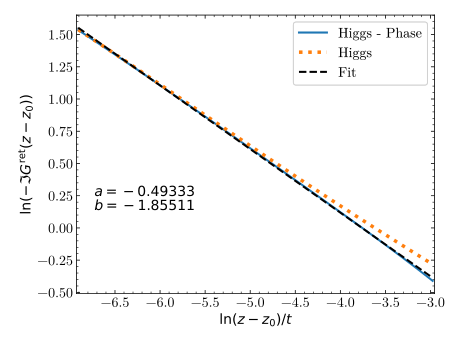
\includegraphics[width=.98\textwidth]{plots/higgs_peak.pdf}
    \caption{Log-log plot of $\spectral{Higgs}$ (a, c) and $\spectral{CDW}$ (b) near $\omega = \omega_0 = 2\Delta_\text{SC}$ at $U=-2.5t$ and $V=0$.
    The different panels depict the spectral functions for various ratios of $\Delta_\text{SC}$ to $\Delta_\text{CDW}$.
    We additionally plot the difference between $\spectral{i}$ and $\spectral{Phase}$ and fit it, as we interpret the latter as a background within the two-particle continuum.
    The left (right) panel shows the results for the square (simple cubic) lattice.
    The spectral function behaves as $1 / \sqrt{\omega - 2 \Delta_\text{tot}}$.
    Note, that $\spectral{CDW}$ and $\spectral{Higgs}$ are identical for the choice in panel (c).}
    \label{fig:higgs_peak}
\end{figure*}

\begin{figure*}
    \centering
    \includegraphics[width=0.98\textwidth]{plots/peak_fits.pdf}
    \caption{Log-log plot of the real part of various Green's functions, the labels indicate its type and the text in the panels indicate the phase.
        The results for both lattice types are shown but are qualitatively identical.
        The power-law exponent is $a=-1$ in all cases, indicating that these peaks are $\delta$ distributions.}
        \label{fig:peak_fits}
\end{figure*}

In this appendix section, we show fits to the real and imaginary parts of various Green's functions in the different phases.
All fits are linear of the type $y = ax + b$ in double logarithmic plots, i.e., $a$ describes the power-law behavior of the functions.
Firstly, the real part of $\greens{Phase}$ in the SC phase is shown in panel (a) of \autoref{fig:zero_peaks}.
It behaves as $1/\omega^2$ indicating that the peak we find in the spectral function at $\omega=0$ corresponds to the derivative of a $\delta$ distribution.
The same results are obtained for the peak in $\spectral{Higgs}$ and $\spectral{CDW}$ in the coexistence phase.

Continuing, we investigate the divergence at $\omega = 2\Delta$ found in $\spectral{Higgs}$ and $\spectral{CDW}$ at $V=0$.
It behaves as $1/\sqrt{\omega}$ as shown in \autoref{fig:higgs_peak}.

Lastly, we show all the remaining peaks in \autoref{fig:peak_fits}.
The real part of each one of them behaves as $1/\omega$ in close vicinity to the peak position.
This indicates that the peaks are $\delta$ distributions.
The peaks of $\spectral{AFM}$ and $\spectral{CDW}$ close the the phase transition are identical when swapped, i.e., $\spectral{AFM}$ in the CDW phase is the same as $\spectral{CDW}$ in the AFM phase.

\section{Numerical treatment of the iEoM matrices}
\label{sec:numerical_ieom}

We would like to use operators like \eqref{eqn:ieom_basis_operator} to span our operator set.
However, numerically, it is impossible to matrices with infinite dimensions, requiring us to discretize.
Additionally, we cannot numerically write down $\delta$ distributions as matrix elements. Therefore, we need some special treatments, which we will describe in this section.
We discretize the $\gamma$-space equally with each abscissa $\gamma_i$ being spaced by $\Delta \gamma$.
Then, we define an approximate $\delta$ function
\begin{equation}
    h(\gamma) \coloneqq \begin{cases}
        \frac{1}{\Delta \gamma} & |\gamma| < \frac{\Delta \gamma}{2} \\ 0 & \text{otherwise}
    \end{cases}\,.
\end{equation}
Computing an integral numerically yields
\begin{equation}
    \int f(\tilde{\gamma}) h(\tilde{\gamma} - \gamma_j) \mathrm{d} \tilde{\gamma} \approx \sum_i f(\gamma_i) h(\gamma_i - \gamma_j) \Delta \gamma = f(\gamma_j)\,,
\end{equation}
showing that $h(\gamma)$ mimicks the continuous $\delta$ distribution for a discrete description.
Note, that if one takes the limit $\Delta \gamma \to 0$ the $\delta$ distribution is exactly reproduced.

Numerically, we can compute the matrix elements like this
\begin{equation}
    \label{eqn:numerical_example}
    (A_i | A_j) = \frac{1}{N} \sum_{\vk \vl} h(\gamma_i - \hat{\gamma}(\vk)) h(\gamma_j - \hat{\gamma}(\vl)) (A_{\vk} | A_{\vl})\,.
\end{equation}
Here, all expressions are finite numbers and do not require further treatment.
Mutatis mutandis, one obtains a similar expression for $(A_i | [H, A_j])$.
Additionally, note, that the expressions $(A_{\vk} | A_{\vl})$ and $(A_{\vk} | [H, A_{\vl}])$ can be reduced to sums of terms that are proportional to $\gamma_i$ or $\gamma_j$, respectively.
Therefore, it is not necessary to implement any sort of momentum space computations.
For example, consider $A_{\vk} = f_{\vk}^\dagger$, then
\begin{equation}
    ( f_{\vk}^\dagger | f_{\vl}^\dagger ) = \delta_{\vk, \vl}\, \langle 1 - n_{\vk \uparrow} - n_{\vk \downarrow} \rangle \eqqcolon \delta_{\vk, \vl}\, \alpha(\vk)
\end{equation}
holds. Inserting this into \eqref{eqn:numerical_example} yields
\begin{equation}
    (A_i | A_j) = \frac{1}{N} \sum_{\vk} h(\gamma_i - \hat{\gamma}(\vk)) h(\gamma_j - \hat{\gamma}(\vk)) \alpha(\vk)\,.
\end{equation}
As stated in the main text, see \eqref{eqn:equal_expecs}, $\alpha(\vk)$ depends only on $\hat{\gamma}(\vk)$, hence we can switch from the momentum sum to a $\gamma$ integration
\begin{align}
    (A_i | A_j) &= \int \rho(\gamma) h(\gamma_i - \gamma) h(\gamma_j - \gamma) \alpha(\gamma) \dgamma \nonumber \\
        &\approx \rho(\gamma_i) h(\gamma_j - \gamma_i) \alpha(\gamma_i) \nonumber \\
        &= \frac{\delta_{ij}}{\Delta \gamma} \rho(\gamma_i) \alpha(\gamma_i)\,.
\end{align}
Since $\Delta \gamma$ is a positive constant factor, it does not impact any of our matrix operations, i.e., we can pull it out to the front of the expressions $\mM \to \tilde{m} (\Delta \gamma)^2$ and $\mN \to \tilde{n} (\Delta \gamma)^2$.
Then, we can rewrite \eqref{eqn:green_derivation} as
\begin{equation}
    G_{AB^\dagger}(z) = - (\Delta \gamma)^2 \vec{b}^\dagger (0) \left[ \tilde{n} \frac{1}{\tilde{m} + z \tilde{n}} \tilde{n} \right] \vec{a}(0)\,.
\end{equation}

To give a practical example, let us compute $\greens{Higgs}$ from \eqref{eqn:resolvent_bases}.
We order our operator set such that all $f_\gamma + f_\gamma^{\dagger}$ are upfront. 
This requires the vector elements $\vec{a}$ and $\vec{b}$ to be
\begin{equation}
    a_i = b_i = \begin{cases}
        1 & i < N_\gamma \\
        0 & \text{otherwise}
    \end{cases}\,,
\end{equation}
where $N_\gamma$ is the number of discretization points.
Using this, we can expand the relation for the Green's function
\begin{align}
    \greens{Higgs} (z) &= -(\Delta \gamma)^2 \sum_{i=0}^{N_\gamma} \sum_{j=0}^{N_\gamma} \left[ \tilde{n} \frac{1}{\tilde{m} + z \tilde{n}} \tilde{n} \right]_{ij} \nonumber \\
        &\approx - \int \dgamma \int \dgamma' \left[ \tilde{n} \frac{1}{\tilde{m} + z \tilde{n}} \tilde{n} \right](\gamma, \gamma')\,.
\end{align}
The first line is an approximation of the integral in the second line, as each matrix element corresponds to a specific value for $\gamma$.

\section{Antisymmetry of the spectral functions}
\label{sec:antisymmetry_spectral}

Consider any Hermitian operator $A$. 
We compute the Fourier-transformed Green's function for positive and negative $\omega$
\begin{align}
    G_{AA}(\omega) &= -i \int_0^\infty e^{i \omega t} \langle [A(t), A] \rangle \mathrm{d}t\,, \nonumber \\
    G_{AA}(- \omega) &= -i \int_0^\infty e^{-i \omega t} \langle [A(t), A] \rangle \mathrm{d}t\,.
\end{align}
We also compute the complex conjugate of the former
\begin{align}
    G_{AA}^* (\omega) &= i \int_0^\infty e^{-i \omega t} \langle [A(t), A] \rangle^* \mathrm{d}t \nonumber \\
        &= i \int_0^\infty e^{-i \omega t} \langle [A^\dagger, A^\dagger(t)] \rangle \\
        &= -i \int_0^\infty e^{-i \omega t} \langle [A(t), A] \rangle \\
        &= G_{AA}(- \omega)
\end{align}
Taking the imaginary part reveals
\begin{align}
    \Im [ G_{AA}^* (\omega) ] = - \Im [G_{AA} (\omega) ] = \Im [G_{AA} (-\omega)]\,.
\end{align}
This proves that the imaginary part of such a Fourier-transformed Green's function is antisymmetrical and therefore the same applies to the spectral functions.
Note, that this fully abides by the sum rule $\int_{-\infty}^\infty \mathcal{A}_{A^\dagger A} (\omega) \mathrm{d}\omega = \langle [A^\dagger, A] \rangle = 0$ \cite{rickayzen80}.



\bibliography{sn-bibliography}
%\bibliography{../../A_bibinput/liter10.bib}
		
\end{document}
